\chapter{Macchina di Turing}
\section{Introduzione}Si cerca di catalogare dal punto di vista computazionale i \textbf{problemi
  intrattabili}, ovvero problemi risolvibili ma non in modo \textbf{efficiente}
(ovvero in tempo polinomiale). In alcuni casi si pensa che non esista una
soluzione ma non si hanno dimostrazioni in merito mentre in altri casi è
addirittura dimostrato. Abbiamo quindi delle categorie informali per i problemi:
\begin{itemize}
  \item \textbf{facili}, so risolverli in modo efficiente. È la \textbf{classe P}
  \item \textbf{difficili} o, più formalmente, \textbf{intrattabile}, so
  risolverli ma non in modo efficiente e non abbiamo una 
  dimostrazione che mi assicuri che non siano risolvibili in modo efficiente. È
  la \textbf{classe NP} e la sua sottoclasse \textbf{NP-complete}
  \item \textbf{dimostrabilmente difficili}, so risolverli ma so che non esiste
  un algoritmo efficiente in quanto è stato dimostrato che non può esistere
  \item \textbf{impossibili}, non so risolverli sempre neanche in modo non
  efficiente (esiste almeno un \textit{input} che manda in crisi l'algoritmo ma esiste
  almeno un caso in cui funzioni)
\end{itemize}
Come formalismo useremo la \textbf{Macchina di Turing (\textit{TM})},
\textit{deterministica} e \textit{non deterministica}. Analizzeremo in primis
\textbf{problemi sui grafi}. 
\subsection{Esempi sui problemi intrattabili e facili.}
\begin{esempio}
	Considero il problema \emph{arco minimo}. Come parametro abbiamo un grafo pesato
	sugli archi $G=(V,E)$. Le proprietà della soluzione è che voglio l'arco con
	peso minimo.\\
	Per risolvere guardo tutti gli archi è vedo quello di peso minimo. Dato che
	basta iterare su tutti gli archi quindi la soluzione è in $O(n)$ (in realtà
	$\Theta(n)$), quindi in \textbf{tempo lineare} sul numero di archi (è quindi
	in \textbf{tempo polinomiale}). Questo è un problema della classe P.
\end{esempio}
\begin{esempio}
	Considero il problema \emph{raggiungibilità}. Come parametro abbiamo un grafo non
	pesato $G=(V,E)$ e due vertici, uno sorgente e uno destinazione, tali che
	$v_s,v_d\in V$. Le proprietà della soluzione è che voglio sapere se posso
	arrivare a $v_d$ partendo da $v_s$.\\
	Per risolvere studio tutti i cammini che partono da $v_s$ e posso dare la
	risposta. Una soluzione del genere è in tempo $O(2^{|E|})$. Il tempo quindi
	cresce in \textbf{modo esponenziale}. Una soluzione migliore è quella di usare
	un \textbf{algoritmo di visita} che richiede tempo $O(|V|+|E|)$, ovvero un
	\textbf{tempo polinomiale}. Quindi per quanto all'inizio si pensi
	che sia un \textbf{problema intrattabile} si scopre che è un \textbf{problema
	facile} (classe P).
\end{esempio}
\begin{esempio}
	Considero il problema \emph{TSP}. Come parametro abbiamo un grafo pesato sugli
	archi e completo $G=(V,E)$. Le proprietà della soluzione è che voglio sapere
	il \emph{cammino minimo} (in realtà un ciclo) che tocca tutti i vertici una e
	una sola volta (una volta trovata la soluzione non mi interessa la sorgente
	essendo il grafo completo). \\
	Sarebbe facile determinare \textbf{un} ciclo ma non quello di peso minimo e
	per farlo devo trovare tutti i cicli e trovare quello di peso minimo. abbiamo
	quindi un algoritmo che è $O(2^n)$ (nella realtà è circa $O(n!)$ che è
	comunque esponenziale per l'\textbf{approssimazione di Stirling}). In questo
	caso non si riesce a pensare ad una soluzione che non sia esponenziale nel
	tempo (anche se per alcuni \textit{input} sia di facile risoluzione, basti pensare ad
	avere tutti gli archi di peso 1, ma mi basta avere un \textit{input} problematico). Non
	potendo però dimostrare che sia irrisolvibile si dice che è un
	\textbf{problema intrattabile}. \textit{TSP} è uno dei 10 problemi famosi per
	i quali ti danno un milione di dollari se dimostri che è o \emph{facile} o
	\emph{impossibile}
\end{esempio}

\subsection{Una prima definizione di Algoritmo}
Per completezza definiamo un \textbf{algoritmo} come una sequenza di
\textbf{istruzioni elementari} (supportate dal calcolatore) che, eseguite in
sequenza, mi portano alla soluzione di un problema. Si ha quindi che un
algoritmo $A$ risolve un problema $\Pi$ se per ogni possibile istanza di $\Pi$
l'algoritmo $A$ mi dà la risposta corretta. Distinguo però:
\begin{itemize}
	\item \textbf{algoritmo efficiente}, che mi dà la soluzione in \textbf{tempo
	      polinomiale} rispetto alla \textbf{dimensione dell'\textit{input}}. abbiamo un
	\textit{caso peggiore} limitato superiormente da un \textbf{polinomiale}:
	$O(p(n))$. abbiamo una crescita di tempo accettabile all'aumentare
	dell'\textit{input}. Diciamo comunque che è dura anche solo raggiungere $O(n^{10})$
	quindi anche se dire polinomiale potrebbe voler dire $O(n^{10000000})$ non si
	hanno casi reali di questo tipo. Un problema della classe P (facile) si risolve con un algoritmo efficiente.
		  
	\item \textbf{algoritmo non efficiente}, che mi da la soluzione ma in tempo
	      superiore a quello \textbf{polinomiale}. abbiamo un \textit{caso peggiore} limitato
	      superiormente da un \textbf{esponenziale}: $O(2^n)$. abbiamo una crescita di tempo
	      assolutamente non accettabile (esponenziale appunto) all'aumentare dell'\textit{input}. Un problema intrattabile o dimostralmente difficile si risolve con un algoritmo non efficiente.
\end{itemize}
\textit{Se abbiamo anche solo un caso di \textit{input} che porta a tempo esponenziale abbiamo
	comunque un algoritmo non efficiente}.\\

\section{Problemi intrattabili}
Ci serve a questo punto una definizione più rigorosa di \textbf{algoritmo}, per
poterne calcolare meglio i tempi. Ricordiamo che per assunzione un algoritmo è
\textbf{efficiente} se viene eseguito in tempo polinomiale rispetto alla dimensione
dell'\textit{input} $x$. Un algoritmo esponenziale è un
algoritmo \textbf{non efficiente}, il tempo cresce troppo velocemente
all'aumentare dell'\textit{input} (anche se magari in alcuni casi non è in tempo
esponenziale). Si ricorda che si studia sempre il tempo nel 
\textbf{caso peggiore}, prenderemo quindi sempre l'O-grande sulla dimensione
dell'\textit{input} $O(f(x))$.\\
Vediamo degli esempi:
\begin{itemize}
  \item un algoritmo che cerca l'arco minimo lavora in tempo polinomiale nel
  caso peggiore ed è quindi un \textbf{problema trattabile}
  \item problemi, come il test di primalità o TSP, che non hanno un algoritmo
  polinomiale sono \textbf{intrattabili}, infatti nessuno ha mai dimostrato che
  esiste un algoritmo efficiente
\end{itemize}
Tra i problemi intrattabili abbiamo però problemi che sono
\textbf{dimostrabilmente intrattabili}. Banalmente un problema che mi chiede di
stampare tutte le possibili sequenze per una certa proprietà è in questa
categoria, dovendo stampare tutte le sequenze possibili si ha $O(2^n)$ e si può
dimostrare che con meno operazioni non si stamperebbero alcune soluzioni
corrette.\\
Ci concentreremo su problemi intrattabili ma non \textit{dimostrabilmente
  intrattabili}.\\
Per anni problemi come il \textit{test di primalità} potevano garantire che
prima o poi si sarebbe trovato un algoritmo polinomiale. Quindi abbiamo:
\begin{itemize}
  \item Problemi dimostrabilmente intrattabili.
  \item Problemi non dimostrabilmente intrattabili, sono, diciamo, ``i più
  difficili'' tra i problemi intrattabili.
  \item Tutti gli altri problemi.
\end{itemize}
\begin{nota}
un problema indecidibile non è un problema intrattabile, in quanto non
si hanno proprio algoritmi che risolvono un certo problema e questo è
dimostrabile (c'è almeno un \textit{input} che manda in crisi un algoritmo, che va in
loop infinito o sbaglia risposta) mentre un problema intrattabile comunque in
qualche modo lo posso risolvere ma in tempi troppo elevati.
\end{nota}
\begin{shaded}
  L'algoritmo per il test di primalità funziona in $\log (n^{12})$, nella
  versione più efficiente sviluppata da un gruppo d'indiani, che arriva ad
  ottenere un tempo polinomiale.
\end{shaded}
\section{Definizione della TM}
Definiamo quindi in modo più rigoroso il concetto di algoritmo per poter
dimostrare che un certo algoritmo può anche non esistere. Non ci basta più la
definizione di algoritmo come sequenza di passi logici, in quanto andrebbe anche
definito un certo linguaggio (con scelte, cicli, operazioni aritmetiche,
operazioni logiche) ma ancora non basterebbe, non si è ancora sicuri di poter
trasformare un certo \textit{input} in un certo \textit{output} (per qualunque problema in
\textit{input}). Lo step mancante è la \textbf{macchina di Turing}, con essa si può
garantire quanto appena detto, con essa si formalizza il processo di calcolo,
ovvero la serie di passaggi che porta da un \textit{input} ad un \textit{output}. Turing ragionò
dicendo che normalmente si risolve un problema partendo da carta e penna,
ponendosi poi in un certo stato mentale in cui si risolve o si studia una parte
dell'\textit{input} (ad esempio in uno stato \textit{leggi tutti} leggo ``step by step''
tutto l'\textit{input}, senza cambiare stato mentale, che verrà cambiato quando finisco
quello precedente). Divide quindi l'\textit{input} in \textit{caselle} su cui si fanno
operazioni semplici, spostandosi a destra o a sinistra di una casella, o
leggendo/scrivendo la casella corrente. Turing ipotizza di avere carta
illimitata. Quindi la MT avrà un nastro infinito che permette di memorizzare
informazioni e si ha una testina di lettura e scrittura. Si ha un meccanismo che
si pone in uno \textit{stato}, sulla base del contenuto letto dalla testina e
dallo stato posso scegliere di spostarmi di una testina a destra o di una a
sinistra, eventualmente dopo avere scritto e modificando, sempre eventualmente,
lo stato. Tutto questo basta per il \textbf{calcolo}, infatti:
\begin{definizione}[Tesi di Turing-Church]
  Non esiste nessun formalismo di calcolo che sia più
  potente della Macchina di Turing:
  \begin{center}
   ``Se un problema è umanamente calcolabile, allora esisterà una macchina di
    Turing in grado di risolverlo''
  \end{center}
  È una tesi che non ha dimostrazione formale (non avendo chiara la definizione
  di \textbf{calcolo}) ma è stata dimostrata
  empiricamente nel corso degli anni, portando quindi a dire che il calcolo è tutto
  ciò che può essere eseguito (o computato) con una Macchina di Turing.\\
  
\end{definizione}
\begin{figure}
  \centering
  \begin{tikzpicture}
    \tikzstyle{every path}=[very thick]

    \edef\sizetape{0.7cm}
    \tikzstyle{tmtape}=[draw,minimum size=\sizetape]
    \tikzstyle{tmhead}=[arrow box,draw,minimum size=.5cm,arrow box
    arrows={east:.25cm, west:0.25cm}]
    \begin{scope}[start chain=1 going right,node distance=-0.15mm]
    \node [on chain=1,tmtape,draw=none] {$\ldots$};
    \node [on chain=1,tmtape] {};
    \node [on chain=1,tmtape] {$\triangleright$};
    \node [on chain=1,tmtape] (input) {b};
    \node [on chain=1,tmtape] {b};
    \node [on chain=1,tmtape] {a};
    \node [on chain=1,tmtape] {a};
    \node [on chain=1,tmtape] {a};
    \node [on chain=1,tmtape] {a};
    \node [on chain=1,tmtape] {$\sqcup$};
    \node [on chain=1,tmtape,draw=none] {$\ldots$};
    \node [on chain=1] {\textbf{\textit{input}/\textit{output} Tape}};
\end{scope}
  \end{tikzpicture}
  \caption{Esempio di nastro di una TM}
  \label{fig:tur}
\end{figure}
\subsection{Formalizzazione di una TM}
Formalizziamo quindi la macchina di Turing.
\begin{definizione}
  Si definisce formalmente una TM come la quintupla:
  \[TM=(K,\Sigma,k_0, \delta, F)\]
  \begin{itemize}
    \item insieme $K$ di stati
    \item un alfabeto $\Sigma$
    \item uno stato di partenza $k_0$
    \item una funzione di transizione $\delta$
    \item un insieme $F$ di stati finali
  \end{itemize}
  Si hanno inoltre i seguenti stati finali:
  \begin{itemize}
    \item $H$, per l'\textit{halt}
    \item $Y$, per lo \textit{yes}
    \item $N$, per il \textit{no}
  \end{itemize}
  Il simbolo $\sqcup$ specifica che non abbiamo un simbolo e il simbolo
  $\triangleright$ mi specifica che da lì parte l'\textit{input}.
\end{definizione}
\subsubsection{Funzione di Transizione}
\begin{definizione}
  La funzione di transizione esprime cosa fa passo-passo la TM:
  \[\delta:K\times\Sigma\to K\times \Sigma\times\{\leftarrow,\rightarrow,-\}\]
  Prevede in \textit{input} uno stato e un simbolo, e in \textit{output} un cambio
  di stato, di simbolo, e lo spostamento della testina. 
  Gli \textit{output} della TM possono cambiare come rimanere invariati.\\
  Avere questa funzione di transazione comporta l'avere una
  \textbf{TM deterministica}, da cui si potrà sviluppare una \textbf{TM non
    deterministica}.
\end{definizione}
Ogni operazione sulla TM impiega lo stesso tempo e perciò posso usare il numero di
operazioni per calcolare il tempo di risoluzione.\\
Per esprimere la computazione di una TM usiamo una \textbf{configurazione},
ovvero definisco tutti i passaggi che la mia TM deve svolgere partendo da uno stato iniziale, 
fino ad arrivare ad uno stato di accettazione.

\subsubsection{Configurazione di una TM}
\begin{definizione}
  Un \textbf{configurazione} di una TM è definita da:
  \begin{itemize}
    \item Lo stato in cui si trova.
    \item La stringa presente sul nastro, definita dall'insieme di tutti i simboli presenti a destra della testina, cui vanno aggiunti tutti quelli presenti a sinistra conteggiando anche quello corrente presente sotto la testina. 
    \item La posizione delle testina. 
  \end{itemize}
  In base alla configurazione la TM saprà come procedere.\\
  La configurazione descrive in ogni istante lo stato della macchina, avendo per una stringa generica $S$ la seguente \textbf{configurazione iniziale}:
  \[(k_0,\triangleright S, 1)\]
  il carattere $\triangleright$ viene aggiunto come carattere di \textbf{start}.
  Ad un certo punto si arriverà ad uno stato di arresto, per esempio dopo
  aver cambiato $S$ in $S1$ ed esser andati nella posizione due:
  \[(H,\triangleright S1, 2)\]
  ottenendo la stringa $S1$, senza il $\triangleright$, che diverrà il mio \textit{output}.\\
   Potremmo avere anche come \textit{output} $Y$ (yes) o $N$ (no) al posto di $H$ (halt) in problemi decisionali.
\end{definizione}
\subsubsection{Esempi di TM}
Vediamo alcuni esempi di costruzione di TM:
\begin{esempio}
  Si scriva la TM che calcoli il successore di un numero binario, che sarà
  l'\textit{input} (e si dà per scontato che sia correttamente formattato avendo solo 0 o
  1 come simboli). Si trascuri il riporto (nel senso che non aggiungo ulteriori
  bit).\\
  \begin{shaded}
    Vediamo nella pratica un esempio di somma binaria:\\
    prendo $01101010$ e sommo uno:
    \[10010101 \, +\]
    \[00000001=\]
    \[\rule{70pt}{.4pt}\]
    \[10010110\,\,\,\,\,\,\,\]
  \end{shaded}
  Definisco quindi la TM:
  \begin{itemize}
    \item $S=\{s_0,s_1\}$
    \item $\Sigma =\{\triangleright, \sqcup, 0,1\}$
    \item Per la funzione di transizione si ha:
    \[\delta\to(s_0,[\triangleright, 0,1])\to(s_0,[\triangleright, 0,1],
      \rightarrow)\]
    \[\delta\to(s_0,\sqcup)\to(s_1,\sqcup,\leftarrow)\]
    \[\delta\to(s_1,0)\to(H,1,-)\]
    \[\delta\to(s_1,1)\to(s_1,0,\leftarrow)\]
    \[\delta\to(s_1,\triangleright)\to(H,\triangleright,-)\]

    ovvero scorro fino alla fine e inverto l'ultimo numero, il quale se è zero diventa uno garantendomi 
    l'arresto della TM, mentre se è uno lo rendo zero e mi continuo a spostare verso sinistra in cerca di
    uno zero che mi garantisca la terminazione.
  \end{itemize}
    \item $s_0$ è lo stato iniziale
\end{esempio}
A un certo punto si arriva allo stato finale $H$. In quel momento abbiamo
una nuova stringa $S1$, contenente il risultato delle mie modifiche su $S$:
\[(H,\triangleright S1, -)\]
La testina, non dovendo più spostarsi, può essere interpretato come uno \textbf{stato di arresto}.\\
Un altro caso è avere una computazione infinita nel caso in cui, letto un
simbolo e lo stato, la testina ricopia il simbolo ma non si sposta ne a destra
ne a sinistra. Oppure una testina potrebbe ``rimbalzare'' infinitamente tra due
posizioni. Quest'ultima cosa può anche accadere tra molte posizioni, entrando
comunque in \textbf{loop infinito} \footnote{Un insieme \textbf{finito} di elementi (stati, simboli e transizioni) può comunque descrivere un comportamento \textbf{infinito} (insieme infinito di passi)}, ritornando sempre, prima o poi, in una
configurazione (e si noti ``configurazione'', non coppia stato-simbolo) già
avuta. In questo caso la computazione è \textbf{non terminante} e la
computazione non produce alcun \textit{output}. \\

Analizziamo meglio gli stati terminanti $Y$ e $N$: il primo indicante che la
stringa in \textit{input} è accettata, avendo certe caratteristiche richieste, il secondo
che la stringa viene rifiutata. Non abbiamo più bisogno della stringa in
\textit{output}, quindi posso lasciar scritto quello che voglio quando finisco, mi basta
sapere lo stato finale $Y$ e $N$.
\begin{esempio}
  Sistemiamo l'esempio precedente aggiungendo il riporto, dovendo aggiungere un
  bit. \\
 \textit{Si indica solo la funzione di transizione}.\\
  Scorro fino alla fine (quindi vado a destra indipendentemente dal simbolo fino
  a un blank):
  \[\delta\to(s_0,[\triangleright, 0,1])\to(s_0,[\triangleright, 0,1],
    \rightarrow)\]
  Sono a destra dell'ultimo carattere di $X$ (avendo un blank):
  \[\delta\to(s_0,\sqcup)\to(s_1,\sqcup,\leftarrow)\]
  eseguo il conto tornando indietro:
  \[\delta\to(s_1,0)\to(H,1,-)\]
  \[\delta\to(s_1,1)\to(s_1,0,\leftarrow)\]
  sono tornato all'inizio:
  \[\delta\to(s_1,\triangleright)\to(s_2,1,\leftarrow)\]
  devo ``shiftare'' tutti i caratteri (per farlo semplicemente metto
  $\triangleright$ nel primo blank a sinistra del precedente $\triangleright$
  arrivando nello stato $s_2$, come indicato nello step precedente):
  \[\delta\to(s_2,\sqcup)\to(H,\triangleright,-)\]
  (avrei comunque potuto shiftare tutte le unità a destra di una posizione, o
  semplicemente, sapendo che ora sul nastro abbiamo soli 0 dovrei tornare a destra di
  un passo, cambiare il primo 0 in 1 e aggiungere uno 0 in fondo alla
  stringa).
\end{esempio}
\begin{esempio}
  Vediamo un esempio in cui una TM riconosce se una stringa binaria è
  palindroma o meno.\\
  \textit{Si indica solo la funzione di transizione}.\\
  Se sono sullo start vado a destra di uno:
  \[\delta(s_0,\triangleright)\to (s_0,\triangleright, \rightarrow)\]
  se vedo 0 vado nello stato $zero$, scrivo $\sqcup$ e vado a destra:
  \[\delta(s_0,0)\to (zero,\sqcup, \rightarrow)\]
  analogo leggendo 1, andando nello stato $1$ scrivendo blank:
  \[\delta(s_0,1)\to (one,\sqcup, \rightarrow)\]
  vado in fondo alla stringa (qualsiasi incrocio tra gli stati $one$ e $zero $ e
  simboli 1 e 0 legga vado a destra riscrivendo lo stesso simbolo):
  \[\delta\to([zero, one],[0,1])\to(\delta\to([zero, one],[0,1],\rightarrow)\]
  sono in fondo alla stringa, se sono in stato $zero$ scrivo blank e torno
  indietro, in uno stato $zero'$:
  \[\delta(zero, \sqcup)\to(zero', \sqcup, \leftarrow)\]
  idem per stato $one$
  \[\delta(one, \sqcup)\to(one', \sqcup, \leftarrow)\]
  se sono in $zero'$ e leggo $0$ vado in stato $s_1$ e vado a sinistra: 
  \[\delta(zero', 0)\to(s_1,\sqcup, \leftarrow)\]
  se sono in $zero'$ e leggo $1$ la stringa non è palindroma, esco con stato
  $N$:
  \[\delta(zero', 1)\to(N,\sqcup, \leftarrow)\]
  idem per stato $one'$, andando in stato $s_2$:
  \[\delta(one', 1)\to(s_2,\sqcup, \leftarrow)\]
  \[\delta(one', 0)\to(N,\sqcup, \leftarrow)\]
  ora proseguo a sinistra fino ad un blank riscrivendo quanto letto:
  \[\delta(s_1,[0,1])\to(s_1,[0,1], \leftarrow)\]
  sono nel blank e torno allo stato iniziale, potendo ricominciare la
  computazione:
  \[\delta(s_1,\sqcup)\to(s_0,\sqcup, \rightarrow)\]
  ma se la stringa (di cardinalità pari) è palindroma cancello tutto, devo
  quindi specificare che se in $s_0$ abbiamo blank la stringa è valida:
  \[\delta(s_0,\sqcup)\to(Y, \sqcup,-)\]
  se invece la stringa è di cardinalità dispari, allo stato attuale, entra in
  loop, dobbiamo quindi aggiungere un uscita da $zero'$ o $one'$ in questo
  caso:
  \[\delta([zero',one'], \sqcup)\to(Y, \sqcup, -)\]
\end{esempio}
\begin{esempio}
  Scrivo una TM per decidere se la stringa in \textit{input} è del tipo $a^nb^nc^n$.\\
  \textit{Si indica solo la funzione di transizione}.\\
  Se leggo $a$ vado nello stato $A$ e vado a destra
  \[\delta(s_0,a)\to (A,\sqcup, \rightarrow)\]
  Se leggo in $s_0$ $b$ o $c$ significa che non abbiamo $a$ quindi esco:
  \[\delta(s_0,[b,c])\to (N,\sqcup, -)\]
  Se in $A$  troviamo un'altra $a$ la lascio e vado a destra:
  \[\delta(A,a)\to (A,a', \rightarrow)\]
  Se in $A$ leggo $b$ vado in $B$, e vado a destra:
  \[\delta(A,b)\to (B,b', \rightarrow)\]
  se invece leggo $c$ non abbiamo $b$ e esco:
  \[\delta(A,c)\to (N,\sqcup, -)\]
  se in $B$ e  troviamo $a$ non va bene:
  \[\delta(B,a)\to (N,\sqcup, -)\]
  Se in $B$  troviamo un'altra $b$ la lascio e vado a destra:
  \[\delta(B,b)\to (B,b, \rightarrow)\]
  Se in $B$ leggo $c$ vado in $C$ e vado a sinistra a controllare:
  \[\delta(B,c)\to (C,c', \leftarrow)\]
  controllo tramite i sentinella indicati con $'$.\\
  Siamo in $C$ quindi:
  \[\delta(C,c')\to (C,c', \leftarrow)\]
  Se però vedo $b$ o $b'$ resto in $C$ e riscrivo:
  \[\delta(C,[b,b'])\to (C,[b,b'], \leftarrow)\]
  Per $A$ cambia, se vedo $a$ scorro:
  \[\delta(C,a)\to (C,a, \leftarrow)\]
  ma se vedo $a'$ torno in $s_0$:
  \[\delta(C,a')\to (s_0,a', \rightarrow)\]
  ma ora $A$ può incontrare $b'$, che va bene, o $c'$ che non va bene:
  \[\delta(A,b')\to (A,b', \rightarrow)\]
  \[\delta(A,c')\to (N,\sqcup, -)\]
  Per $C$:
  \[\delta(C,[b,c])\to (C,[b,c'], \rightarrow)\]
  Se sono in $s_0$ e  troviamo $a'$ abbiamo finito le $a$:
  \[\delta(s_0,a')\to (s_0,a' , \rightarrow)\]
  idem:
  \[\delta(s_0,[b',c')\to (s_0,[b',c'] , \rightarrow)\]
  Vado in stato $check$ se:
  \[\delta(s_0,\sqcup)\to(check,\sqcup, \leftarrow)\]
  e proseguo fino a trovare solo $b'$ o $c'$, se  troviamo invece $b$ o $c$ esco.
  Diventa quindi molto lungo.
\end{esempio}
L'esempio sopra mostra quanto possa diventare lunga una semplice computazione
sulla TM, ci servirebbe quindi una sorta di \textit{TM alternativa}.
\subsubsection{TM multi-nastro}
\begin{definizione}[definizione di B\"{o}hm-Jacopini]
  Qualunque algoritmo può essere implementato utilizzando tre sole strutture, la
  sequenza, la selezione e il ciclo, da applicare ricorsivamente alla
  composizione d'istruzioni elementari
\end{definizione}
\begin{definizione}
  Si ha la \textbf{TM a $k$ nastri}, ovvero la \textbf{TM
    multi-nastro} dove abbiamo $k$ nastri di lettura e scrittura, magari avendo
  l'\textit{input} solo su un nastro o su multipli. La macchina quindi legge uno stato e
  $k$ simboli $\{\sigma_1\ldots,\sigma_k\}$. Prima dello spostamento quindi
  scrive tutti i simboli. Lo spostamento sarà uno per ogni nastro.
\end{definizione}
\begin{esempio}
  Risolviamo il precedente problema (decidere se la stringa in \textit{input} è del tipo
  $a^nb^nc^n | n\geq0$) con $k$ nastri.\\
   Potremmo usare quattro nastri, sul primo c'è l'\textit{input}. Finché  troviamo "a" scrivo sul
  primo, quando  troviamo "b" passo a secondo e faccio l'analogo se leggo "c". In
  ogni caso mi interrompo se dopo delle "b"  troviamo "a" o dopo "c"  troviamo
  "a,b". Infine torno indietro sui tre nastri e vedo se sono allineati.
    \[\delta(s_0,\triangleright, \sqcup, \sqcup, \sqcup)\to (s_0, \triangleright , \sqcup, \sqcup, \sqcup, \rightarrow, -, - ,-)\]
    Caso stringa vuota:
    \[\delta(s_0,\sqcup, \sqcup, \sqcup, \sqcup)\to (Y, \sqcup , \sqcup, \sqcup, \sqcup, \rightarrow, -, -, -)\]
    Inserisco le $a$ sul secondo nastro:
    \[\delta(s_0, a, \sqcup, \sqcup, \sqcup)\to (s_a, a , a, \sqcup, \sqcup, \rightarrow, \rightarrow, -, -)\]
    \[\delta(s_0, b, \sqcup, \sqcup, \sqcup)\to (N, \sqcup, \sqcup, \sqcup, \sqcup, -, -, -, -)\]
    \[\delta(s_0, c, \sqcup, \sqcup, \sqcup)\to (N, \sqcup, \sqcup, \sqcup, \sqcup, -, -, -, -)\]
    \[\delta(s_a, a, \sqcup, \sqcup, \sqcup)\to (s_a, a, a, \sqcup, \sqcup, \rightarrow, \rightarrow, -, -)\]
    Inserisco le $b$ sul terzo nastro:
    \[\delta(s_a, b, \sqcup, \sqcup, \sqcup)\to (s_b, b, \sqcup, b, \sqcup, \rightarrow,  -, \rightarrow, -)\]
    \[\delta(s_a, c, \sqcup, \sqcup, \sqcup)\to (N, \sqcup, \sqcup, \sqcup, \sqcup, -, -, -, -)\]
    \[\delta(s_a, \sqcup, \sqcup, \sqcup, \sqcup)\to (N, \sqcup, \sqcup, \sqcup, \sqcup, -, -, -, -)\]
    \[\delta(s_b, a, \sqcup, \sqcup, \sqcup)\to (N, \sqcup, \sqcup, \sqcup, \sqcup, -, -, -, -)\]
    \[\delta(s_b, \sqcup, \sqcup, \sqcup, \sqcup)\to (N, \sqcup, \sqcup, \sqcup, \sqcup, -, -, -, -)\]
    \[\delta(s_b, b, \sqcup, \sqcup, \sqcup)\to (s_b, b, \sqcup, b, \sqcup, \rightarrow, -, \rightarrow, -)\]
    Inserisco le $c$ sul quarto nastro:
    \[\delta(s_b, c, \sqcup, \sqcup, \sqcup)\to (s_c, c, \sqcup, \sqcup, c, \rightarrow, -, -, \rightarrow)\]
    \[\delta(s_c, a, \sqcup, \sqcup, \sqcup)\to (N, \sqcup, \sqcup, \sqcup, \sqcup, -, -, -, -)\]
    \[\delta(s_c, b, \sqcup, \sqcup, \sqcup)\to (N, \sqcup, \sqcup, \sqcup, \sqcup, -, -, -, -)\]
    \[\delta(s_c, \sqcup, \sqcup, \sqcup, \sqcup)\to (N, \sqcup, \sqcup, \sqcup, \sqcup, -, -, -, -)\]
    \[\delta(s_c, c, \sqcup, \sqcup, \sqcup)\to (s_c, c, \sqcup, \sqcup, c, \rightarrow, -, -, \rightarrow)\]
    Faccio un passo indietro sui nastri (e continuo così ricorsivamente):
    \[\delta(s_c, \sqcup, \sqcup, \sqcup, \sqcup)\to (s_f, \sqcup, \sqcup, \sqcup, \sqcup, -, \leftarrow, \leftarrow, \leftarrow)\]
    \[\delta(s_f, /, a, b, c)\to (s_c, /, \sqcup, \sqcup, \sqcup, -, \leftarrow, \leftarrow, \leftarrow)\]
    \[\delta(s_f, /, \sqcup, \sqcup, \sqcup)\to (Y, \sqcup, \sqcup, \sqcup, \sqcup, -, -, -, -)\]
    \[\delta(s_f, /, a, \sqcup, \sqcup)\to (N, \sqcup, \sqcup, \sqcup, \sqcup, -, -, -, -)\]
    ... tutte le rimanenti combinazioni che portano a uno stato N.
\end{esempio}
Una \textbf{TM a $k$ nastri} non è più potente di una \textbf{TM a singolo
  nastro} (vale il rapporto linguaggio di programmazione e linguaggio
macchina). Esiste sempre una traduzione verso la TM a singolo nastro.\\
Per esempio invece un automa a stati finiti è meno potente di un TM, che può
spostarsi e scrivere dove vuole, a differenza degli automi.\\
\subsection{Decisione e Accettazione di una TM}
Vediamo cosa quindi può fare una TM:
\begin{itemize}
  \item Una TM può \textbf{computare} funzioni su stringhe.
  \item Una TM può \textbf{decidere} (rispondendo $Y$ o $N$) un linguaggio
  (ovvero un insieme finito o infinito di stringhe, come il caso sopra
  $a^nb^nc^n$), ovvero data una stringa in \textit{input} è sempre in grado di dire se  appartiene o meno a un dato linguaggio.
  \item Una TM può \textbf{accettare} un linguaggio, ovvero: fornendo una stringa in \textit{input}, appartenente al linguaggio, la TM la riconosce come tale e prima o poi arriva nello stato $Y$, altrimenti la macchina potrebbe:
  \begin{itemize}
    \item Fermarsi in uno stato $N$.
    \item Entrare in un loop infinito (poiché si è passata in \textit{input} una stringa che NON appartiene al linguaggio, che ricordiamo, è quasi sempre INFINITO), il quale può essere realmente infinito, oppure finito ed estremamente oneroso in termini di tempo. Tuttavia non è possibile capire a priori quale delle due ipotesi è giusta quando ci si trova in questa casistica.
  \end{itemize}
\end{itemize}
\section{I Linguaggi}
I linguaggi possono essere:
\begin{enumerate}
    \item Ricorsivi
    \item \textbf{NON} Ricorsivi
    \item Ricorsivamente enumerabili
    \item \textbf{NON} Ricorsivamente enumerabili
\end{enumerate} 
\begin{definizione}
  Un linguaggio è \textbf{ricorsivo}, se esiste
  almeno una TM che riesce a deciderlo, fermandosi sempre in $Y$ o
  $N$ . Solitamente è un linguaggio finito, ma potrebbe anche essere infinito (ma
  tutte le stringhe sarebbero comunque riconoscibili). Essi sono collegati ai problemi \textbf{decidibili}.
\end{definizione}
 \begin{definizione}
   Un linguaggio è \textbf{ricorsivamente enumerabile} se, data una stringa opportuna in
  \textit{input}, la TM restituisce $Y$, altrimenti la TM potrebbe o fermarsi con $N$ o andare
  avanti all'infinito nella computazione. Posso enumerare tutte le stringhe che
  fanno parte del linguaggio tramite una procedura specifica.  Potremmo avere
  un linguaggio finito ma con 
  stringhe che mandano in loop la TM, anche se comunque non sono in grado di
  capire se sono in un loop o se prima o poi la stringa data in \textit{input} verrà
  riconosciuta.
 \end{definizione}
Dato l'alfabeto $\Sigma$, presa la chiusura
di $\Sigma$ (che mi descrive tutte quelle stringhe ottenibili concatenando zero o N simboli di $\Sigma$), ovvero $\Sigma^*$,
la TM riconosce subito la stringa in \textit{input} in quanto costruita per funzionare
su $\Sigma$, quindi il linguaggio è ricorsivo. Se prendo $\Sigma^+$, ovvero
$\Sigma^*$ senza $\varepsilon$, abbiamo comunque un linguaggio ricorsivo per lo
stesso motivo, dovendo solo controllare in più se $s_0$ è $\sqcup$.\\
 \begin{nota}
 Un linguaggio finito è ricorsivo.
 \end{nota} 
 \begin{definizione}
  Preso un linguaggio $L$ costruito su un alfabeto $\Sigma$. Preso $L\subseteq\Sigma^*$ se $L$ è ricorsivo allora è ricorsivamente
  enumerabile.
\[L\,\,\in\,\,R \implies L\,\,\in\,\,RE\]
\end{definizione}
\begin{proof}
    Se $L$ è ricorsivo esiste una TM che riconosce se, data una stringa $x$,
    $x\in L$ rispondendo $Y$, o $N$ altrimenti (Poiché il problema è decidibile).\\
    Presa una TM $M'$ per cui se il linguaggio non fosse ricorsivo allora entra
    in loop (quest`ultimo indicato con $\infty,\uparrow,\bot$). Quindi quando la macchina sta
    per andare in $N$ cambio $\delta$ per ottenere il loop, ottenendo una
    macchina che va in loop se $x\not\in L$, mentre riconosce con $Y$ se $x\in
    L$ e quindi $L$ è ricorsivamente enumerabile. 
  \end{proof}
\begin{definizione}
  $L$ è ricorsivo sse $L$ è ricorsivamente enumerabile e il complementare di
  $L$ ($\overline{L}$) è ricorsivamente enumerabile.
  \[L\,\,\in\,\,R \iff L\,\,\in\,\,RE\,\,\land\,\,\overline{L}\,\,\in\,\,RE\]
\end{definizione}
\begin{proof}
  Rispetto alla dimostrazione precedente, che garantisce che se $L$ è ricorsivo
  allora è ricorsivamente enumerabile, devo definire, per il complementare, una
  TM che va in loop se $x\in L$, andando altrimenti in loop. Presa quindi una TM
  $M$ che decide $L$, definisco $M'$ che accetta $L$, che quindi è
  ricorsivamente enumerabile. Definisco ora $M''$ che restituisce $Y$ se $x\in
  \overline{L}$ ovvero $x\not\in L$ (e $\infty$ se $x\not\in \overline{L}$,
  ovvero $x\in L$). Quindi $M''$ fa la stessa cosa di $M$ ma quando $M$ sta
  per rispondere $Y$ faccio andare $M''$ in loop e se $M$ va in $N$ faccio
  andare $M''$ in $Y$, tutto tramite un cambio di $\delta$.
\end{proof}

\section{Problemi di decisione}
\begin{definizione}
  Un problema di decisione è un problema con solo due possibili risposte, $Y$ e
  $N$ (Quindi il linguaggio associato è ricorsivo).\\
  I problemi di decisione sono restrizioni di problemi di ottimo, ai quali viene
  aggiunto un \textbf{bound}, cambiando la domanda in una richiesta di esistenza
  di un caso che soddisfi la nuova restrizione.
\end{definizione}
\begin{definizione}
  Posso associare un problema di decisione allo studio di un linguaggio, avendo
essi la stessa risposta, $Y$ o $N$. Un problema di decisione ha quindi un
corrispondente linguaggio, con l'\textit{input} del problema che ha una corrispondente
stringa (di cui bisogna studiare l'appartenenza a un linguaggio).
\end{definizione}
\begin{esempio}
  Il problema \textbf{Hamiltonian cycle problem (\textit{HCP})} (esiste anche la
  variante non con il ciclo ma con il cammino: \textbf{Hamiltonian path problem
    (\textit{HPP})}).\\ 
  Dato un grafo non completo e non pesato ci si chiede se c'è un modo per
  partire da un nodo e tornarci dopo aver toccato tutti i vertici una e una sola
  volta.\\
  Questo problema è di decisione ed è risolvibile, ma è difficile da risolvere
  in termini temporali (restringersi ai problemi decisionali non sempre implica
  miglioramenti in termini di tempo). HCP si risolve solo in tempo esponenziale.
\end{esempio}
\begin{definizione}
  Se il problema di decisione non è risolvibile in modo efficiente sicuramente
  il problema di ottimo associato non è risolvibile in modo efficiente.
\end{definizione}
\subsection{Passaggio da un problema decisionale a un linguaggio}
\begin{definizione}
  Preso $\pi$ problema di decisione. Posso passare da $\pi$ a un linguaggio
  $L(\pi)$ attraverso uno \textbf{schema di codifica}, che prende in \textit{input}
  un'istanza $I$ del problema è mette in \textit{output} una stringa del linguaggio. Se
  istanza ha risposta $Y$ abbiamo $cod(I)\in L$ , quindi la stringa appartiene al linguaggio. Se risponde $N$ abbiamo $cod(I)\not\in
  L$, con $cod$ che indica una 
  \textbf{codifica}, ovvero una traduzione dell'istanza nel linguaggio.\\
\end{definizione}
Risolvere un problema di decisione vuole dire essere in grado di riconoscere o meno le stringhe del corrispondente linguaggio.
\begin{definizione}
  Un Problema è \textbf{DECIDIBILE} se il linguaggio associato è \textbf{RICORSIVO}. 
\end{definizione}
\begin{definizione}
  Un Problema è \textbf{INDECIDIBILE} se il linguaggio associato è \textbf{NON RICORSIVO}. 
\end{definizione}
\begin{esempio}
  Pensando a HCP abbiamo:
  \[L_{HCP}=\{y\in \Sigma^*|\mbox{ che corrispondono ad un'istanza con risposta
      Y}\}\]
  Sapendo che HCP è risolvibile so che esiste una TM che risolve il problema e
  il grafo può essere tradotto in stringa, ad esempio tramite una matrice di
  adiacenza.\\
  HCP è risolvile sse il linguaggio associato è decidibile, e quindi ricorsivo.
\end{esempio}
\begin{definizione}
  Il tempo di esecuzione di una TM è il conto dei passi di esecuzione nel caso
  peggiore.
\end{definizione}
\newpage
\subsection{Problemi indecidibili}
I problemi indecidibili, come già descritto precedentemente, sono tali \textbf{sse} il linguaggio associato \textbf{NON} è ricorsivo.
\[\pi \,\, non\,\,decidibile\,\, \iff L(\pi)\,\,non \,\,ricorsivo\]
\subsubsection{Universal Turing Machine}
\begin{definizione}
  Definiamo la \textbf{Universal Turing Machine (\textit{UTM})} come una TM che
  non fa un compito specifico in base alla $\delta$ ma prende in \textit{input} un'altra
  TM $M$, un separatore ``;'' e l'\textit{input} $x$ di $M$ e da in \textit{output} la stessa cosa
  che darebbe $M$ con \textit{input} $x$:
  \[UTM(M;x)\to M(x)\]
  Quindi calcola quello che calcola qualunque altra TM.
\end{definizione}
La UTM è simile a quello che fa tramite un linguaggio di programmazione, dove si dà una sequenza d'istruzioni e un \textit{input}, ottenendo un \textit{output}. Un calcolatore moderno è quindi una sorta di UTM (con l'hdd che corrisponde al nastro infinito, non avendo potenzialmente limite potendo aggiungere altri dischi).\\ Normalmente si ha che $UTM(M;x)$ ha due nastri: sul primo $(M;x)$ e sul secondo la configurazione attuale di $(M;x)$. Quindi una TM può simularne un'altra salvando le configurazioni. La UTM tramite la sua $\delta$ poi copia lo stato di uscita di $M$, magari scrivendo su un terzo nastro l'\textit{output}.\\ \textbf{Posso quindi costruire una TM (la UTM) che simuli un'altra TM}, quindi si è in grado di scrivere un algoritmo che prende in \textit{input} un altro programma scritto nello stesso linguaggio, che fa le stesse cose, e quindi il primo algoritmo, per esempio, può dare le risposte opposte.\\
\subsubsection{Linguaggi non Ricorsivi e Problemi indecidibili}
\begin{definizione}
  Esistono \textbf{linguaggi non ricorsivi}, ovvero esistono \textbf{problemi indecidibili} (come i dieci problemi proposti da Hilbert a inizio novecento).
\end{definizione}
Ci sono problemi che possono essere chiaramente descritti per i quali sappiamo
che non esiste alcun algoritmo in grado di risolverli (di risolverli
\textbf{sempre}, basta quindi anche solo un caso per cui non posso avere tale algoritmo). 
\begin{definizione}
  Un problema non decidibile non è un problema intrattabile,che sarebbe risolvibile ma solo in tempo esponenziale.
\end{definizione}
\subsubsection{Halting problem}
Turing riconosce da subito come interessante l'\textbf{halting problem}. Si
cerca un algoritmo che data una certa coppia $(M;x)$, TM/\textit{input}, mi dica se
quella macchina arriva a termine computazione o entra in loop infinito.
\begin{definizione}
  Definisco formalmente l'\textbf{halting problem} con il linguaggio $H$:
  \[H=\{M;x|\,M(x)\neq\bot\}\]
  Quindi se la stringa fa parte del linguaggio $M$ termina, altrimenti no.
\end{definizione}
\begin{definizione}
  Si ottiene però che $H$ non è ricorsivo e quindi l'halting problem non è
  decidibile.
\end{definizione}
\begin{proof}
  Immaginiamo per assurdo che $H$ sia ricorsivo e quindi esiste una TM $T_H(M;x)$ tale che:
  \[T_H(M;x) =
    \begin{cases}
      Y& \mbox{ se }M(x)\neq \bot\\
      N& \mbox{ se }M(x) = \bot
      \label{MH}
    \end{cases}
  \]
  Quindi fa qualcosa in più della UTM, perché se finisce in loop deve capire che
  è in loop infinito, interrompere e restituire $N$.\\
  Assumo che $H$ quindi è ricorsivo e quindi $T_H$ esiste, anche se magari non
  la so costruire. Se esiste $T_H$ deve esisterne un'altra, chiamata $D$, che
  presa in \textit{input} solo $M$ produce:
  \[D(M)\to T_H(M;M)\]
  Questo significa che esiste una macchina $D$ che \textbf{simula} la macchina $T_H$ \textbf{non} su \textit{input} generico ma dando in \textit{input} la descrizione di M stessa. Significa che un programma prende in \textit{input} se stesso (che comunque è una stringa). In particolare, secondo le ipotesi di $T_H$ (fig \ref{MH}):
  \[T_H(M;M)= D(M) = 
    \begin{cases}
      Y& \mbox{ se }M(M)\neq \bot\\
      N& \mbox{ se }M(M)=\bot
    \end{cases}
  \]
  Ora voglio far si che la macchina $D$, non solo simuli $T_H$, ma ne inverta anche i risulati. Quindi $D$ cambia $N$ in $Y$ e $Y$ in $\infty$, presa in \textit{input} una macchina
  $M$:
    \[D(M) = T_{Hinvertita}(M;M) =
    \begin{cases}
      Y& \mbox{ se }M(M) = \bot\\
      \bot& \mbox{ se }M(M)\neq \bot
    \end{cases}
  \]
  Provo quindi a dare in \textit{input} a $D$ se stessa, quindi per come è stata teorizzata la macchina avremo:
  \[T_{Hinvertita}(D;D) = D(D) = 
    \begin{cases}
      Y& \mbox{ se }T_H(D;D) = N\\
      \bot & \mbox{ se }T_H(D;D) = Y
    \end{cases}
  \]
  Analizziamo più nel dettaglio i casi in cui $D(D)$ valga $\bot$ o $Y$:
    \[D(D) = 
    \begin{cases}
      Y& \mbox{ se }T_H(D;D) = N \implies D(D) = \bot\\
      \bot & \mbox{ se }T_H(D;D) = Y  \implies D(D) \neq\bot
    \end{cases}
  \]
  Siamo arrivati all'assurdo.  \\
  \[D\,\,\,non\,\,\,esiste\,\,\,\implies\,\,\,T_H\,\,\,non\,\,\,esiste\,\,\,\implies\,\,\,H\,\,\,non\,\,\,è\,\,\,ricorsivo.\]
\end{proof}
Si è dimostrato quindi che anche problemi ben definiti possono non essere
decidibili, problemi come il definire il comportamento di un programma dato un
\textit{input}. Il problema comunque non è una potenza limitata della TM ma un limite
intrinseco al problema stesso. \\ Abbiamo verificato che una TM non può dimostrare che un programma termina o va in loop, però possiamo dimostrare che esiste una TM che dimostra solo se un programma termina.
\begin{definizione}
  Il linguaggio $H$ è ricorsivamente enumerabile, ovvero il problema è
  \textbf{parzialmente decidibile}. La macchina quindi riconosce una macchina
  che termina, altrimenti non si sa.  
\end{definizione}
\begin{proof}
  Devo trovare una macchina che termina in $Y$ che riconosce una stringa
  appartenente al linguaggio $H$.\\
  Costruisco quindi una $T_H'$ che prende in \textit{input} una TM generica col suo
  \textit{input} e si ha che:
  \[T_H'(M;x)=
   \begin{cases}
     Y &\mbox{ se } M(x)\mbox{ termina}\\
     N/\infty &\mbox{ altrimenti}
    \end{cases}
  \]
  Quindi se non termina non si sa che succede, ma potrebbe anche essere sempre
  in loop.\\
  Pensando a UTM abbiamo che:
  \[UTM(M;x)=
   \begin{cases}
     Y &\mbox{ se } M(x)=Y\mbox{ avendo }T_H'=Y\\
     N &\mbox{ se } M(x)=N\mbox{ avendo }T_H'=Y\\
     H &\mbox{ se } M(x)=H\mbox{ avendo }T_H'=Y\\
     \infty &\mbox{ se } M(x)=\infty\mbox{ avendo }T_H'=\infty\\
    \end{cases}
  \]
  Quindi $T_H'$ è una UTM con gli stati finali leggermente modificati (quindi
  non più una UTM), avendo
  solo $Y$ (se termina) e $\infty$ (altrimenti). Abbiamo quindi dimostrato che è
  \textbf{parzialmente decidibile}, avendo che la macchina da $Y$ se la
  computazione è terminante e va in loop altrimenti.
\end{proof}
Ho quindi problemi indecidibili che sono parzialmente decidibili. Esistono
anche problemi legati a linguaggi \textbf{non ricorsivamente enumerabili}, per
cui quindi non si può \textbf{mai} dare risposta. Si hanno quindi problemi
nemmeno parzialmente decidibili. Pensiamo alle coppie $(M;x)$ che non terminano.
\begin{definizione}
   Esistono linguaggi \textbf{non ricorsivamente enumerabili} avendo quindi
   problemi indecidibili.
\end{definizione}
\begin{proof}
  Basti pensare che se $L$ è ricorsivo sse $L$ e $\overline{L}$ sono ricorsivamente
  enumerabili. Quindi, pensando all'halting problem, $L_H$ non è ricorsivo ma
  è ricorsivamente enumerabile. Ma allora $\overline{L_H}$, il linguaggio
  complementare non è ricorsivamente enumerabile: 
  \[\overline{L_H}=\{M;x|M(x)=\bot)\]
\end{proof}
\subsection{Problemi decidibili}
I problemi decidibili, come già descritto precedentemente, sono tali \textbf{sse} il linguaggio associato è ricorsivo.
\[\pi \,\,decidibile\,\, \iff L(\pi)\,\,ricorsivo\]
Studiamo ora i problemi decidibili catalogandoli in base ai tempi, nei casi
peggiori. Come già ampiamente spiegato, si possono risolvere mediante diverse tipologie di algoritmi: 
\begin{itemize}
  \item \textbf{Trattabili}: algoritmi in tempo polinomiale rispetto alla dimensione dell'\textit{input}
    \item \textbf{Intrattabili}: algoritmi in tempo esponenziale rispetto alla dimensione dell'\textit{input} ma non si è ancora dimostrato l'inesistenza di algoritmi polinomiali che li risolvono.
  \item \textbf{Dimostrabilmente intrattabili}: algoritmi in tempo esponenziale rispetto alla dimensione dell'\textit{input}.
\end{itemize}
Il tempo di esecuzione viene calcolato tramite il numero di passi della TM.
\subsubsection{Calcolo del tempo}
\begin{definizione}
  Definiamo $t_M(x)$ come il tempo di calcolo di un TM $M$ su \textit{input} $x$. \textbf{Non è
  un caso peggiore ma è relativo al singolo \textit{input} specifico}. Il tempo di
  calcolo è il numero di passi che esegue $M$ su \textit{input} $x$ per dare una
  risposta. Concentrandosi sui problemi di decisione decidibili avrò sempre $Y$
  o $N$ se $x$ fa parte o meno del linguaggio. Ci concentriamo solo sui
  linguaggi ricorsivi.
\end{definizione}
\begin{nota}

Non si usa comunque il numero di passi nella realtà ma si usa l'O-grande,
studiando il caso peggiore, il numero massimo di passi. Questo aspetto verrà analizzato nel prossimo capitolo.
\end{nota}
\begin{definizione}
  Definiamo $T_M(n)$ come la \textbf{funzione di complessità temporale} come:
  \[T_M(n)=\max\{t_m(x)|\,|x|=n\}\]
\end{definizione}
\subsubsection{Calcolo dello spazio}
\begin{definizione}
  Definisco lo \textbf{spazio di calcolo} come $s_M(x)$, ovvero il numero di celle del nastro visitate dalla TM $M$ con \textit{input} $x$ durante la computazione.
\end{definizione}
\begin{definizione}
  Definisco $S_M(n)$ come la \textbf{funzione di complessità spaziale}:
  \[S_M(n)=\max\{s_M(x)|\,|x|=n\}\]
\end{definizione}
\subsubsection{Legame tra Spazio e Tempo}
Spazio e tempo sono legati per una TM.\\
Innanzitutto se una computazione dura $n$ passi (tempo) posso dire che al più abbiamo
usato $n$ celle (spazio), perché magari in qualche passo la testina rimane ferma
ma nel caso peggiore si sposta sempre. Si ha quindi:
\[S_M(n)\leq T_M(n)+n\]
con $+n$ perché sul nastro abbiamo comunque l'\textit{input} di lunghezza $n$ (anche se
potrebbe non essere letto dalla TM). In alcuni casi non viene nemmeno
considerato come spazio usato in quanto non cambia la risposta in merito agli
studi di tempo (a meno di studiare tempi inferiori al tempo lineare, dove in
caso si specifica a parte di avere un \textit{input} che occupa spazio $n$).
\begin{definizione}
  Se il tempo è limitato allora lo spazio è limitato ma non vale l'opposto
  ( potremmo avere banalmente un loop tra poche celle, avendo l'uso limitato di
  poche celle per un tempo illimitato).
\end{definizione}
\begin{definizione}
  Se abbiamo una TM $M$ che lavora in spazio finito e tempo infinito, esiste una TM
  $M'$ che fa la stessa cosa di $M$ in tempo limitato.\\
  Quindi se lo spazio è limitato allora posso costruire un'altra TM in cui il tempo è limitato.
\end{definizione}
\begin{proof}
  La macchina $M'$ può trovarsi in un numero finito di stati $K$ e, avendo spazio limitato, possiede un numero limitato $S_M(n)$ di celle in cui si può ritrovare la testina. $M'$ possiede anche un numero finito di simboli in alfabeto $\sigma$ e quindi: 
  \[T_{M'}(n)\leq|k|\cdot |S_M(n)|\cdot |\Sigma|^{|S_M(n)|}\]
  dove:   \[ |\Sigma|^{|S_M(n)|} \] indica che posso scrivere una quantità di $\sigma$ simboli per $S_M(n)$ caselle.
  da ciò si evince che prima o poi si ritorna in stati già visti quindi la macchina se supera
  la quantità appena definita capisce di essere in loop (questo perché si ha a
  che fare con insiemi limitati e quindi tale ragionamento non va bene per
  l'halting problem).
\end{proof}
Quindi data una certa macchina che lavora in un certo spazio $S(n)$ posso
costruire una macchina equivalente che da la stessa risposta in tempo limitato
$T(n)$. Si ha che se abbiamo un problema che si risolve in spazio polinomiale, per
la formula appena scritta avrò tempo esponenziale. Invece, al contrario, tempo
polinomiale comporta spazio polinomiale.
\section{La Classe P: Deterministic Turing Machine}
\begin{definizione}
  Definisco la classe $P$ in base alle TM. La \textbf{classe P} è definita come:
  \[P=\{L|\mbox{ L è deciso da una DTM in tempo polinomiale } O(p(n))\}\]
  Con DTM che indica una TM deterministica, in cui per ogni coppia stato/simbolo
  la macchina può fare una sola cosa (leggere/*scrivere/spostarsi di uno)m e con
  $p$ una certa funzione polinomiale.\\
  È quindi la classe di problemi che so risolvere velocemente.
\end{definizione}
\begin{definizione}
  Definiamo la classe \textbf{\textit{time(f(n))}} come la classe dei linguaggi
  decisi da una TM entro un tempo $f(n)$. Quindi \textbf{\textit{time(n)}} sono
  tutti quelli decisi in tempo lineare, ad esempio (ma  potremmo anche per un
  qualsiasi $n^k$).\\
  Quindi:
  \[P=\cup_{i\geq 0} time(n^i)\]
  Infatti $P$ è l'unione di tutte le classi \textit{time} con funzioni
  polinomiali. 
\end{definizione}
\begin{definizione}
  Se un problema è nella \textbf{classe P} allora è risolvibile in un
  \textbf{tempo efficiente}.
\end{definizione}
\section{NonDeterministic Turing Machine}
I problemi nella \textbf{classe EXP} sono ancora in studio per capire se sono
\textbf{dimostrabilmente intrattabili}. Per il loro studio
si usano le \textbf{NonDeterministic Turing Machine (NDTM)} che sono comunque
puramente teoriche, in quanto non si è in grado fisicamente di costruirle. 
\subsection{Relazione di Transizione}
Nella DTM deterministica abbiamo una $\delta$ mentre nella NDTM abbiamo:
\[\Delta\subseteq (k\times \Sigma)\times (k\times \Sigma \times\{\leftarrow,
  \rightarrow, -\})\]
Con $\Delta$, detta \textbf{relazione di transizione}, che non è una funzione
(come era $\delta$) ma una relazione.\\ 
Nella DTM dato uno stato potevo passare a un solo stato tramite $\delta$,
passando di stato in stato fino a uno stato finale. Era una sequenza di
transizioni. \\
Nella NDTM abbiamo delle \textbf{scelte}, ovvero la computazione non è una sequenza
di computazioni ma un \textbf{albero di computazione}. Da ogni stato posso
passare a uno tra più stati, a seconda della \textit{scelta}, formando così un
albero. Il singolo passo di computazione non è univocamente definito. Ogni
singolo ramo comunque è equivalente al passo di computazione della DTM. Tramite
$\Delta$ definisco il passaggio tra stati.\\
\subsection{Accettabilità e Decidibilità}
Per capire se una stringa è accettata o meno dalla NDTM, visto che  potremmo andare
sia in $Y$ che in $N$ (che in $H$) a seconda della varie computazioni
dell'albero, si ha che:
\begin{definizione}
  Una stringa $x$ è \textbf{accettata} da una NDTM se esiste una computazione
  tale per cui:
  \[(s_0,x,1)\to(Y, z, \rho_G)\]
  quindi se almeno un ramo dell'albero di computazione che termina nello stato
  $Y$. Tutti gli altri rami possono fare quello che vogliono, anche restare in
  loop.\\
  Se non c'è almeno un ramo $Y$ non è accettata. Gli altri possono andare in
  loop o in uno stato $N$.
\end{definizione}
\begin{definizione}
  Un linguaggio $L$ è \textbf{accettato} da una NDTM $N$ se per tutte le
  stringhe che fanno parte del linguaggio esiste \textbf{almeno} una computazione che
  termina nello stato $Y$, ovvero esiste una computazione per cui:
  \[\forall x\in L\Rightarrow \exists\,\,almeno\,\, una\,\, computazione\,\, di\,\, N\,\, con\,\, \textit{input}\,\, x\,\, tale\,\, che\,\, N(x)=Y\]
\end{definizione}
\begin{definizione}
  Un linguaggio $L$ è \textbf{deciso} da una NDTM $N$ se, qualora la stringa $x$
  appartenga al linguaggio, esiste \textbf{almeno una} computazione tale per
  cui: 
  \[x\in L\rightarrow N(x)=Y\]
  altrimenti, se $x$ non appartiene al linguaggio, per \textbf{tutte} le
  computazioni, si ha che: 
  \[x\not\in L \rightarrow N(x)=N\]
  Non devo quindi avere loop in questo caso, tutte devono dare $N$.
\end{definizione}
\begin{esempio}
  Si ha:
  \[L=\{a^nb^{2n}\}\cup\{a^{2n}b^n\}\]
  Studiamo una DTM che riconosca tale linguaggio. Dalle DTM controlla prima il
  primo formato senza cambiare i simboli. Se vede che le $a$ sono più delle $b$
  passo al secondo step, dopo aver riconvertito i simboli in $a$ e $b$. Dopo
  aver analizzato il secondo insieme restituisce $Y$ o $N$. Tale funzione di
  transazione non è scontata.\\
  Una NDTM potrebbe essere:
  \[(s_0,x,1)\]
  che va in
  \begin{itemize}
    \item $(s_1,x,1)$, da cui parte lo studio del primo insieme
    \item $(s_2,x,2)$, da cui parte lo studio del secondo insieme
  \end{itemize}
  Data una stringa che non fa parte di $L$ tutti i rami terminano con
  $N$. Altrimenti almeno un ramo porta a $Y$ a seconda dei tipi di stringa
  accettati, se appartengono al primo o al secondo insieme. \\
  La scelta del ramo non è definita formalmente, è solo una \textit{scelta}. La
  macchina sa il ramo da scegliere dopo aver analizzato la stringa iniziale.
\end{esempio}
\begin{definizione}
  Una NDTM non è ``più potente'' di una DTM in termini di capacità di
  riconoscimento di un linguaggio. Se abbiamo una NDTM che accetta un linguaggio
  sicuramente abbiamo una DTM che lo fa. Le NDTM sono ``più potenti'' in termini di tempo di computazione.
\end{definizione}
\begin{proof}
  La NDTM non viene simulata da una DTM procedendo per rami, concludendoli, ma
  si procede per singoli passi su ogni ramo (onde evitare d'incappare
  prematuramente in loop). Si scende quindi per livelli simulando poi tutti i
  rami (dovendo però ``tornare indietro'' ogni volta per passare al ramo
  successivo). Quindi muovendomi tra i rami posso simulare tramite una DTM
  quanto fa una NDTM.
\end{proof}
\begin{definizione}
  La NDTM $N$ decide il linguaggio $L$ in tempo $T(N)$ se:
  \begin{itemize}
    \item $N$ decide $L$
    \item $\forall\,x\in \Sigma^*$ se la macchina $M$ effettua $k$ passi del tipo $(s_0,x,1)\to(s_G, z, \rho_G)$ in modo tale che $k\leq F(N)$
  \end{itemize}
  Quindi, se la stringa fa parte del linguaggio, la macchina la riconosce come tale poiché la \textbf{decide} in, al massimo, $F(N)$ passi . Altrimenti, se la stringa non fa parte del linguaggio, la macchina lo deve capire in, al massimo, $F(N)$ passi.
\end{definizione}
In un modo la $NDTM$ riesce a capire quale strada percorrere, in al più $F(N)$ passi, per trovare $Y$ (altrimenti la risposta è $N$, poiché non si potrebbe andare il loop essendo l'albero limitato da $F(N)$). Si può pensare come una macchina \textbf{parallela}, che segue ogni livello di ogni ramo in concorrenza.
Quindi la NTDM, per quanto non più potente in termini di riconoscimento, lo è in
base al tempo, basandosi sui livelli dell'albero.
\subsection{Classe NP}
La classe di problemi \textbf{NP} (\textbf{NON-DETERMINISTIC POLYNOMIAL TIME}) è una classe di complessità usata per classificare problemi decisionali. NP è un insieme di problemi decisionali in cui le istanze la cui risposta è "yes" sono verificabili in un tempo \textbf{polinomiale} da una TM \textbf{non} deterministica.
Quindi, la classe dei problemi facilmente verificabili di cui non si ha una facile
risoluzione altro non è che la \textbf{classe NP}, che sono problemi polinomiali
in modo non deterministico.
\begin{definizione}
  la \textbf{classe NP} corrisponde all'insieme di linguaggi $L$ che sono decisi
  da una NDTM in tempo polinomiale:
  \[F(n)=O(p(n))\]
\end{definizione}
Si ha un rapporto tra $P$ e $NP$.
\begin{definizione}
  Data una NDTM $N$ che decide $L$ in tempo $F(n)$ esiste una DTM $M$ che decide
  $L$ in tempo $O(d^{F(n)})$, dove $d$ è una caratteristica particolare della
  NDTM, ovvero il \textbf{grado massimo di divisione dell'albero di
    computazione}\footnote{Da Wikipedia: In informatica un albero binario è un albero i cui nodi hanno grado compreso tra 0 e 2. Per albero si intende un grafo non diretto, connesso e aciclico mentre per grado di un nodo si intende il numero di sotto alberi del nodo, che è uguale al numero di figli del nodo.} di $N$. 
\end{definizione}
\begin{proof}
  $M$ ha vari nastri:
  \begin{itemize}
    \item il primo contiene $N$
    \item il secondo simula $N$
    \item il terzo contiene un numero in base $d$, inizialmente $1$
  \end{itemize}
  La macchina fa un passo di simulazione di $N$, andando nel primo ramo ($d=1$)
  a sinistra. A questo punto:
  \begin{itemize}
    \item trova $Y$ e si ferma
    \item trova $N$ quindi va avanti
    \item trova un altro stato, incrementa $d$ e passa al ramo indicato da
    $d$
  \end{itemize}
  e così via. Nello step successivo farà due passi e non uno, per ogni
  ramo. Valutando quindi eventuali nuove ramificazioni per ogni ramo. \\
  Se $N$ arriva a $Y$ allora troverò certamente uno $Y$ per $M$. Se arriva a $N$
  dopo un po' tutti i rami terminano in $N$ ma devo verificare la cosa e a quel
  punto $M$ termina con $N$.\\
  La simulazione richiede $d$ passi per il primo livello, $d^2$ per il secondo,
  $d^i$ per l'i-simo livello. Mi fermo a $d^{F(N)}$, al livello $F(n)$ e quindi
  abbiamo tempo: 
  \[O(d^{F(N)})\]
\end{proof}

\subsection{P, NP ed EXP}
La NDTM è quindi più potente per i tempi, per quanto ne sappiamo infatti che se
la NTDM lavora in $F(n)$, quindi in tempo polinomiale, la DTM che la simula
lavora in $d^{F(n)}$, quindi in tempo esponenziale. Quindi la NDTM è ``più
veloce'', anche se non lo sappiamo con certezza.\\
Rispetto al rapporto tra $P$ e $NP$ possiamo dire che $P\subseteq NP$, in quanto
una NDTM è un caso generale della DTM (dove la relazione non ha mai scelte). Si
ha inoltre che ci sono problemi che non sappiamo dire se sono in $P$ o meno ma sappiamo che sono in $NP$. Allo stesso tempo ci sono problemi che sappiamo essere in $NP$ ma nessuno ha mai trovatola dimostrazione che sia in $P$. (problemi intrattabili).\\
Capire qualcosa in merito ai problemi del secondo tipo potrebbe portare a $P=NP$
o $P\neq NP$. Questo è uno dei 10 problemi aperti della matematica ed è
il più importante per l'informatica teorica.\\
A questo conosciamo quindi $P$, $NP$, $EXP$ (poste in ordine di ``è contenuto
in''):
\[P\subseteq NP \subseteq EXP\]
Anche se $p\subseteq NP$ è al centro di studi.\\
\subsection{Accenni di Riduzioni Polinomiali}
Ordiniamo i problemi in base alla difficoltà in queste due classi, tramite le
\textbf{riduzioni polinomiali} tra problemi (che ipotizziamo solo di decisione per praticità) $A\to B$.
\begin{definizione}
  Una riduzione è una procedura che trasforma ogni istanza del problema $A$ in un'istanza per un problema diverso $B$.
\end{definizione}
Un'istanza di $A$ ($I_A$) ha due risposte, $Y$ o $N$, ma sfruttando una \[f:I_A\to I_B\] si fa sì che $I_A$ sia \textbf{ridotta} a un'istanza $I_B$. Difatti il problema $B$ riesce a interpretare questa istanza e a dare in \textit{output} una risposta compatibile con $A$.\\ Ragionando sulle tempistiche avremo un tempo totale dato da:
\[Riduzione(x) + Algoritmo(B(x))\]
\begin{definizione}[TSP]
  Il problema del commesso viaggiatore (TSP) è uno dei casi di studio tipici dell'informatica teorica e della teoria della complessità computazionale. Il nome nasce dalla sua più tipica rappresentazione: dato un insieme di città, e note le distanze tra ciascuna coppia di esse, trovare il tragitto di minima percorrenza che un commesso viaggiatore deve seguire per visitare tutte le città una ed una sola volta e ritornare alla città di partenza. 
\end{definizione}
\begin{definizione}[Cammino Hamiltoniano]
  Nel campo matematico della teoria dei grafi, un cammino in un grafo (orientato o non orientato) è detto hamiltoniano se esso tocca tutti i vertici del grafo una e una sola volta.
  \begin{corollario}[Ciclo Hamiltoniano]
  Si ha un ciclo hamiltoniano quando in un cammino hamiltoniano esiste un arco che collega l'ultimo vertice con il primo, realizzando così un ciclo che visita tutti i vertici per poi ritornare al punto di partenza. 
  \end{corollario}
  \begin{corollario}[Grafo Hamiltoniano]
  Un grafo che contenga almeno un ciclo hamiltoniano viene detto grafo hamiltoniano. 
  \end{corollario}
\end{definizione}
Vediamo, ad esempio, se possiamo risolvere il problema del ciclo hamiltoniano
usando TSP, entrambi decisionali. Partendo da un'istanza del grafo per il ciclo
hamiltoniano creo un'istanza con gli stessi vertici, aggiungo gli archi per
ottenere un grafo completo (visto che TSP ha un grafo completo mentre ciclo
hamiltoniano no). Aggiungo anche i pesi (TSP ha un grafo pesato mentre ciclo
hamiltoniano no), mettendo il peso a 1 per i vecchi archi
e $K$, con $k\neq 1$, a quelli appena aggiunti. Manca quindi
solo il bound, che è $B=|V|$ per il ciclo hamiltoniano che ipotizziamo con archi
solo pesati a $1$ ma quindi in TSP non posso usare quelli aggiunti in quanto
uscirei per forza dal bound se usassi uno degli archi aggiunti, basta $K=2$. abbiamo
un ciclo hamiltoniano sse $B=|V|$ anche con TSP, che avrà un giro con gli stessi
archi del ciclo hamiltoniano presente nel primo problema, posto che esista,
avendo che se TSP rende $Y$ sse $B=|V|$ allora avrò un ciclo hamiltoniano nel
problema iniziale, avendo $Y$ in risposta anche per questo. abbiamo quindi ridotto il
ciclo hamiltoniano a TSP, e possiamo dire che quest'ultimo è più difficile di
ciclo hamiltoniano. Per esempio vedere figura \ref{fig:htsp}
\begin{figure}
  \centering
  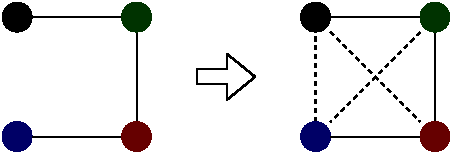
\includegraphics[scale = 0.9]{img/rid.pdf}
  \caption{Esempio di riduzione da ciclo hamiltoniano a TSP, con archi
    tratteggiati di peso 2 e archi normali di peso 1. Il colore dei vertici
    specifica che dalle due parti della trasformazione si ha lo stesso vertice}
  \label{fig:htsp}
\end{figure}
Controlliamo quindi i tempi. Voglio un costo della riduzione polinomiale e si ha
che l'aggiunta di archi, pesi e bound sono operazioni polinomiali.
\begin{definizione}
 Un problema $A$ è difficile \textbf{almeno quanto} un altro problema $B$, che ha in \textit{input} la stringa
  $x$, sse:
  \[A\to B\]
  infatti abbiamo:
  \[T(A(x))\leq F(x)+T(B(x))\]
\end{definizione}
\begin{definizione}
  Definiamo formalmente riduzione polinomiale tra un linguaggio $L_1$ e un
  linguaggio $L_2$ come:
  \[f:\Sigma_1^*\to \Sigma_2^*\]
  tale che:
  \[x\in L_1\iff f(x)\in L_2\]
  con $f$ calcolabile in tempo polinomiale ($O(|x|)$) dalla DTM. SI ha quindi
  che:
  \[L_1<_T L_2\]
  Cioè un problema L1 si riduce a uno L2.
\end{definizione}
\begin{definizione}
  Se si ha che $L_1<_T L_2$ e si ha che $L_2\in P$ allora sicuramente $L_1\in
  P$.\\
  Se avessi avuto $L_2\in NP$ o $L_2\not\in P$ non avrei informazioni su $L_1$. 

\end{definizione}
\begin{proof}
  Infatti esiste un algoritmo polinomiale per $L_2$ allora, avendo una
  trasformazione polinomiale  abbiamo che $f(x)+L_2$ è ancora polinomiale.
\end{proof}
\begin{definizione}
  Se si ha che $L_1<_T L_2$ e si ha che $L_1\not\in P$ allora abbiamo che
  $L_2\not\in P$.
\end{definizione}
\begin{proof}
  Basta vedere ``al contrario'' la definizione precedente.
\end{proof}
\subsubsection{Proprietà delle riduzioni polinomiali}
Le riduzioni godono di proprietà:
\begin{itemize}
  \item riflessiva, $A\to A$
  \item transitiva, $A\to B\,\,\,\land \,\,\,B\to C\implies A\to C$, che essendo
  due trasformazioni in tempo polinomiale avrò comunque una trasformazione
  polinomiale 
\end{itemize}
Le riduzioni polinomiali \textbf{non sono sempre simmetriche} e quindi non sono
una relazione di equivalenza.\\
\subsection{Problemi NP-Complete}
Abbiamo però una classe di equivalenza interna ai problemi NP, dove i problemi
contenuti sono i più difficili di NP e si riducono l'uno all'altro. Tali
problemi sono i problemi \textbf{NP-Complete}.
\begin{definizione}
  Un linguaggio è \textbf{NP-Complete} sse:
  \begin{itemize}
    \item $L\in NP$
    \item $L'<_TL,\forall\,L'\in NP$
  \end{itemize}
  Tutti i linguaggi in NP si riducono a $L\in NP_{complete}$ e quindi i problemi in NP-Complete sono i più difficili di NP.
  Se ne risolvessi uno in tempo polinomiale risolverei tutti i problemi in NP in
  tempo polinomiale.
\end{definizione}
\begin{definizione}
  Per gli NP-Complete vale anche la proprietà \textbf{simmetrica} in quanto ogni problema NP-Complete è riducibile ad ogni altro problema NP-Complete.
\end{definizione}
\subsubsection{Teoremi di NP-Complete}
\begin{definizione}
  $P=NP$ sse esiste un linguaggio $L$ tale che:
  \[L\in NP_{complete}\cap P\]
  Ovvero: esiste un problema NP-Complete in P.
\end{definizione}
\begin{proof}
  Se $P=NP$ allora sappiamo già che sarebbero polinomiali.\\
  Per l'altro verso abbiamo che:
  \[\forall L'\in N, \,\,L<_T L\]
  e quindi esisterebbe un algoritmo polinomiale che risolve L per una DTM e
  quindi avrei un algoritmo polinomiale per ogni $L'\in NP$ per una DTM.
\end{proof}
Quindi se trovassi un algoritmo polinomiale per un NP-Complete lo avrei per
tutti gli NP.
\begin{definizione}
  Se esiste un $L\in NP$ ma $L\not\in P$ allora:
  \[\forall L''\in \mbox{NP-Complete}\implies L''\not\in P \]
Dimostrando quindi che $P\neq NP$.\\
\end{definizione}

Riprendendo l'esempio sopra so
che ciclo hamiltoniano è TSP, anche nelle forme decisionali, e quindi so che TSP
decisionale è NP-Complete. La difficoltà è trovare almeno un problema
NP-Complete, poi saprò che ogni altro a cui posso ridurlo è NP-Complete.\\
\subsubsection{Teorema di Cook}
Conosciamo moltissimi problemi NP-Complete, molti riconosciuti tramite riduzioni
ma il primo è ottenuto tramite il \textbf{definizione di Cook}:
\begin{definizione}[SAT]
  La soddisfacibilità booleana, o soddisfacibilità proposizionale o SAT, è il problema di determinare se una formula booleana è soddisfacibile o insoddisfacibile. La formula si dice soddisfacibile se le variabili possono essere assegnate in modo che la formula assuma il valore di verità vero. Viceversa, si dice insoddisfacibile se tale assegnamento non esiste (pertanto, la funzione espressa dalla formula è identicamente falsa). 
\end{definizione}
\begin{definizione}[Teorema di Cook]
  SAT è NP-Complete. 
\end{definizione}
\begin{proof}
  La dimostrazione completa è complessa ma vediamo qualche spunto.\\
  Si ha che SAT può essere risolto in tempo esponenziale, $O(2^n)$, provando
  tutti i possibili assegnamenti di verità possibili.\\
  Posso usare inoltre una NDTM che fa tutti i rami in parallelo, con ogni
  possibilità di assegnamento fatta in un ramo oppure posso dire che ``spara''
  un assegnamento a caso, che si suppone giusto, su un ramo e verifica che è
  giusto. In ogni caso con una NDTM avrei tempo polinomiale, $O(n\cdot m)$ per
  $n$ variabili e $m$ clausole.\\
  Per vedere che ogni problema NP, per semplicità decisionali, si riduce a SAT
  vedo che tutti i problemi in NP hanno in comune di avere un NDTM che li
  risolve in tempo polinomiale, che decide il linguaggio associato. Basta quindi
  dire che $\forall\Pi'\in NP$ ha associato una NDTM $N_\Pi'$ che lavora in
  tempo polinomiale e mi basta vedere che ogni NDTM che lavora in tempo
  polinomiale si può trasformare in una formula CNF, presa in ingresso da SAT,
  sfruttando poi gli stati finali della computazione di SAT. Se SAT dice che è
  soddisfacibile allora lo è il problema iniziale e quindi il problema è
  riducibile a SAT.
\end{proof}
SAT è stato il primo problema identificato come NP-Complete ed è stato usato per
riconoscere gli altri problemi NP-Complete.\\
La descrizione di una NDTM deve quindi corrispondere ad una $\phi$ di SAT per
far vedere che tutti i problemi NP si riducono a SAT. Si avrà una variabile per
ogni stato, una variabile per ogni carattere e una variabile per la posizione
della testina. Queste variabili saranno quelle che comporranno la $\phi$ e il
loro assegnamento comporterà la veridicità della formula.\\
Bisogna far vedere che $SAT<_T \Pi$ per far vedere che $\Pi$ è
NP-Complete. Facendo poi vedere che un altro problema si riduce a $\Pi$ o SAT
dimostro che anche questo secondo problema è NP-Complete. \\
Si ha che il problema del ciclo hamiltoniano e TSP, decisionali, siano
NP-Complete.\\
Vediamo che $SAT<_T 3SAT$, che ha tre letterali in ogni clausola. abbiamo in \textit{input}
una formula $\phi$ che deve diventare una $\phi_3$ tale che $\phi$ è
soddisfacibile sse $\phi_3$ lo è. La formula $\phi$ ha tante clausole in
congiunzione tra loro con un numero arbitrario di letterali ma $\phi_3$ deve
averne altrettante ma con soli tre letterali per clausola. Qualora si abbiano
clausole in $\phi$ con un solo letterale si aggiungono due letterali (che
indichiamo con $z$) in modo
però che la veridicità sia basata solo sulla variabile iniziale (questo vale per
tutte le trasformazioni che stiamo per mostrare, ovvero la veridicità deve
valere in base solo alle variabili iniziali della formula $\phi$). Tale clausola
che conteneva solo $x_1$ diventa una quadrupla clausola:
\[(x_1\lor z_1\lor z_2)\land (x_1\lor\neg z_1\lor z_2)\land (x_1\lor z_1\lor\neg
  z_2)\land(x_1\lor\neg z_1\lor\neg z_2)\] 
Se invece avessi una formula con due letterali diventa, aggiungendo una sola
variabile: 
\[(x_1\lor x_2\lor z_1)\land (x_1\lor x_2\lor \neg z_1)\]
Una formula a tre letterali resta ovviamente invariata mentre quelle a più
letterali vanno spezzate (aggiungendo poi variabili). Per esempio, avendo
quattro letterali, otterrei:
\[(x_1\lor x_2\lor z_1)\land (\neg z_1\lor x_3\lor z_2)\land (\neg z_2\lor
  x_4\lor z_3)\land\cdots\land(z_{n-3}\lor x_{n-1}\lor x_n)\]
Si vede che ogni formula di SAT può essere trasformata in una di 3SAT e quindi
anche quest'ultimo è NP-Complete. Si dimostra che invece 2SAT non è NP-Complete
ma ogni $K$SAT, con $K>2$, è NP-Complete.\\
Anche, per esempio, il \textit{problema della colorabilità} è NP-Complete, in
quanto può essere ridotto a SAT (non vedremo come).\\
Torniamo a parlare di TSP, non di decisione. abbiamo capito che serve tempo
esponenziale per risolverlo quindi si può pensare che sia NP-Complete. Passo
quindi alla versione di decisione. Vedo però che ciclo
hamiltoniano, che è NP-Complete, si riduce a TSP decisionale che quindi è
anch'esso NP-Complete. Abbiamo comunque che TSP è più difficile del suo problema
decisionale, infatti D-TSP si riduce a TSP. Si ha quindi che TSP è
\textbf{NP-Hard}, ovvero tutti i problemi NP si riducono ad esso ma il problema
stesso non è in NP (essendo un problema di ottimo e quindi non gli posso
associare un linguaggio) e quindi non è NP-Complete (non essendo in NP). Per
TSP servirebbe una \textbf{macchina di Turing ad oracolo}.
\subsection{Rapporto spazio e tempo}
Aggiungiamo qualcosa a quanto già detto nelle sezioni precedenti.\\
\begin{definizione}
  Definisco la \textbf{funzione di complessità spaziale} come:
  \[f:\mathbb{N}\to\mathbb{N}\]
  con $f(n)$ che è il massimo numero di caselle utilizzate da una TM per
  decidere un certo linguaggio $L$ tutte le istanze di una certa dimensione,
  $n=|x|$. 
\end{definizione}
Sappiamo che, dal punto di vista del tempo (in notazione si ha $dtime=time$):
\[P=\bigcup_{k\geq 1}dtime(n^k)\]
\[NP=\bigcup_{k\geq 1}ntime(n^k)\]
\begin{definizione}
  Definiamo la \textbf{classe PSPACE} come l'insieme di tutti i linguaggi tali
  che sono decisi da una TM in spazio $O(f(n))$. Si ha che;
  \[PSPACE=\bigcup_{k\geq 1}dspace(n^k)\]
  avendo quindi limite polinomiale.
\end{definizione}
\begin{definizione}
  Definiamo la \textbf{classe NSPACE} come l'insieme di tutti i linguaggi tali
  che sono decisi da una NDTM in spazio $O(f(n))$. Si ha che:
  \[NPSPACE=\bigcup_{k\geq 1}nspace(n^k)\]
  avendo quindi limite polinomiale.
\end{definizione}
Come vale:
\[P\subseteq NP\]
Vale che:
\[PSPACE\subseteq NPSPACE\]
e per dimostrarlo mi concerto su una macchina che si preoccupa solo dello spazio
e non del tempo.\\
Prendiamo nuovamente il problema SAT e quindi ragioniamo sulla NDTM. Vediamo che
SAT è in NPSPACE per ovvi motivi (capisco che ramo scegliere e tale ramo ha una
casella per letterale, avendo spazio $n$) ma vediamo se appartiene anche a
PSPACE. Una DTM potrebbe provare tutte le possibilità in tempo esponenziale ma
in spazio polinomiale in quanto si sovrascrivono ad ogni tentativo le varie
caselle indicanti gli assegnamenti di verità ma la cardinalità di tali caselle è
sempre la stessa, una per ogni letterale, ovvero $n$. Quindi abbiamo che $SAT\in
PSPACE$ anche se non è un'informazione così eclatante a causa del tempo
esponenziale.
\begin{definizione}[definizione di Savitch]
  Si dimostra che:
  \[PSPACE=NSPACE\]
  Quindi la DTM e la NDTM hanno la stessa potenza dal punto di vista dello
  spazio di calcolo.
\end{definizione}
\begin{proof}
  Un problema abbiamo visto essere definito come \textbf{configurazione
    raggiungibile}, ovvero se una macchina può andare da una configurazione
  iniziale $c_i$ ad una finale $c_f$ in un certo numero di passi $t$, indicato
  con:
  \[(c_i,C_f,t)\]
  Prendo una
  configurazione intermedi $c_m$ e vedo se vale:
  \[\left(c_i,C_m,\frac{t}{2}\right)\land \left(c_m,C_f,\frac{t}{2}\right)\]
  Spezzo poi in modo D\&I di volta in volta, vedendo ricorsivamente se entrambi
  i rami sono validi.\\
  Vedo che lo stack delle chiamate ricorsive ha una certa profondità. Una NDTM
  andrebbe in spazio $f(n)$ ha associata una DTM che lavora in spazio
  $O(f^2(n))$ in quanto salvo le varie configurazioni dello stack ricorsivo,
  avendo $2^{\log f(n)}=f(n)$.\\
  (\textbf{rivedere tutta la dimostrazione, quanto scritto è errato in buona
    parte!})
  
\end{proof}
Abbiamo quindi $PSPACE=NPSPACE$ e che $P\subseteq NP$ quindi certamente:
\[P\subseteq PSPACE\]
\[NP\subseteq NPSPACE\]
Si ha quindi la figura \ref{fig:cla}.
\begin{figure}
  \centering
  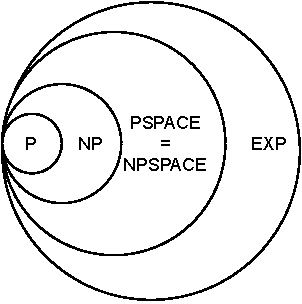
\includegraphics[scale = 0.9]{img/cla.pdf}
  \caption{Diagramma di Venn delle classi fin'ora descritte}
  \label{fig:cla}
\end{figure}
Abbiamo anche le classi $CO\_P$ e $CO\_NP$ ovvero le classi dei problemi
complementari $P$ e $NP$. Si ha che, a causa del determinismo:
\[CO\_P=P\]
ma quando si introduce il non determinismo le cose cambiano. La domanda iniziale
era del tipo \textit{esiste almeno uno} quindi il completamento è \textit{non
  esiste nessuno}, quindi devo verificare tutti i casi, andando in un caso che
nemmeno la NDTM riesce a risolvere, si finisce infatti nella classe
$EXP$. Quindi si ha che:
\[P\subseteq CP\_NP\land P\subseteq NP\]
non avendo un rapporto diretto e definito tra $NP$ e $CO\_NP$.
% \section{Approfondimento Riduzioni polinomiali}
% 			Si hanno alcuni problemi che sono in grado di risolvere qualunque problema di
% 			decisione in \textbf{NP}. Serviranno prima le definizioni di \textbf{NP-Hard} e
% 			\textbf{NP-complete}.\\
% 			Vediamo innanzitutto il problema \textit{independent-set} che ci aiuterà
% 			analisi.
% 			\begin{definizione}
% 				L'\textit{independent-set } di un grafo non orientato è un sottoinsieme
% 				$I\subseteq V$ tale che $\forall u,v\in I$ $(u,v)\not\in E$. Il problema
% 				\textit{ind\_set}, nella versione di ottimo, è quello di trovare
% 				l'\textit{independent-set} di cardinalità massima di un grafo non
% 				orientato. Nella versione di decisione $ind\_set_d$ si ha anche il parametro
% 				$k$ intero e si cerca se esiste un \textit{independent-set} di cardinalità
% 				uguale a $k$. L'\textit{independent-set} di cardinalità massima può essere
% 				usato come ``certificato''.
% 			\end{definizione}
% 			Questo problema è legato alla \textit{copertura dei vertici}, infatti sappiamo
% 			che se dall'insieme dei vertici togliamo un sottoinsieme di minima copertura
% 			troviamo un \textit{independent-set} di cardinalità massima perché sto facendo
% 			il complemento di un insieme di copertura di cardinalità minima, infatti tra i
% 			vertici non nell'insieme di copertura di cardinalità minima, ovvero nel
% 			complemento, non posso avere un arco per definizione e quindi se il primo è di
% 			cardinalità minima allora il secondo, che è l'\textit{independent-set}, è di
% 			cardinalità massima. Infatti i vertici nella copertura sono vertici che toccano
% 			tutti gli archi.\\
% 			Dal punto di vista delle applicazioni pratiche questi problemi si prestano allo
% 			studio, per esempio, delle telecomunicazioni.
% 			\begin{proof}
% 				Dimostriamo che $ind\_set_d$ è \textbf{NP}, infatti esiste un algoritmo $A$
% 				che in costo polinomiale prende in ingresso il grafo, $k$, e un
% 				``certificato'' $y$ e i vertici in $y$, che sono vertici di un
% 				\textit{independent\_set} per il grafo $G$ di cardinalità $k$. L'algoritmo
% 				verifica che $y$ è un \textit{independent-set} e il costo della verifica è
% 				quadratico su $|y|$, ovvero $|y|^2$ che nel caso peggiore è $|V|^2$. So anche
% 				che, per l'\textit{input} $x$, $O(|x|)=O(|E|+|V|)=O(|V^2|+|V|)$ nel caso peggiore,
% 				quindi il tempo di verifica è \textbf{polinomiale}.
% 			\end{proof}
% 			\begin{definizione}
% 				Vediamo ora il problema di \textbf{soddisfacibilità} $SAT$. Questo problema
% 				prende in \textit{input} una formula booleana $\phi$ in \textbf{forma normale congiunta
% 					(CNF)}, ovvero che ha una congiunzione ($\land$) come legame tra le
% 				\textbf{clausole}. Una clausola è un $\lor$ di \textbf{letterali}, ovvero di
% 				variabili booleane $x_i$ o $\neg x_i$. In \textit{output} abbiamo se la forma sia
% 				soddisfacibile o meno. 
% 				\begin{esempio}
% 					Prendo 3 variabili, $x_1,x_2,x_3$. Creo i letterali  $x_1,x_2,x_3$ e anche
% 					$\neg x_1,\neg x_2,\neg x_3$. Creo quindi le clausole $c_1=x_1\lor x_2$,
% 					$c_2=x_1\lor \neg x_2$ e $c_3=x_1\lor \neg x_2$. Definisco quindi la CNF
% 					$\phi$:
										    
% 					\[\phi=(x_1\lor x_2)\land (x_1\lor \neg x_2)\land
% 						(x_1\lor \neg x_2)=c_1\land c_2\land c_3\]
% 						Quindi in ogni clausola almeno un letterale deve essere vero, cosicché tutte
% 						le clausole siano vere rendendo vera la CNF.\\
% 						Avendo due letterali a clausola si è definito un $2SAT$.
% 						\end{esempio}
% 						Il numero di letterali $k$ che compongono la clausola definisce un problema
% 						$kSAT$. Si ha che $2SAT\in P$ ma con $k>2$ si ha che $kSAT\in NP$ (in
% 						realtà è in \textbf{NP-Hard})
% 						\end{definizione}
% 						\begin{definizione}
% 							Definiamo un problema \textbf{NP-Hard} come un problema difficile almeno
% 							quanto un problema \textbf{NP}. Ogni che problema $A$ in \textbf{NP} può
% 							essere risolto con un chiamata di procedura a $B$, che è un problema
% 							\textbf{NP-Hard} a cui tutti gli altri ``chiedono aiuto'' per trovare una
% 							soluzione. \\
% 							Ad esempio \textit{vertex-cover} è un problema \textbf{NP-Hard} e quindi posso
% 							risolvere ogni problema $A$ in \textbf{NP} con il problema
% 							\textit{vertex-cover} $B$.\\
% 							Trasformo quindi l'\textit{input} $w$ di $A$ in un \textit{input}
% 							$f(w)$ per $B$ in tempo polinomiale. La risposta di $B$ con \textit{input} $f(w)$ è la
% 							stessa che $A$ da su \textit{input} $w$.\\
% 							Non tutti i problemi \textbf{NP-Hard} sono dentro la classe \textbf{NP}
% 						\end{definizione}
% 						\begin{definizione}
% 							Definiamo quindi il concetto di \textbf{riduzione}, rappresentato in figura
% 							\ref{fig:rid}.\\
% 							La riduzione è la trasformazione dell'\textit{input} di $w$ in $A$ in un \textit{input} $f(w)$
% 							per $B$, in tempo polinomiale. La risposta di $B$ con \textit{input} $f(w)$ è la stessa
% 							che $A$ da su \textit{input} $w$.\\
% 							Si ha che $A$ si riduce polinomialmente a $B$, e si scrive:
% 							\[A\leq_p B\]
% 							se $\exists\,f$ tale che:
% 							\[w \in L_A\mbox{ sse } f(w)\in L_B\]
% 							con $f$ calcolabile in tempo polinomiale, infatti il calcolo di $f(w)$ è
% 							$=(|w|^p)$, con $p\in\mathbb{N}$ per semplicità. Non devo introdurre una
% 							complessità superiore nel contesto di confronto tra problemi (??).\\ 
% 							\begin{figure}
% 								\centering
																    
% 								\psscalebox{0.9 0.9} % Change this value to rescale the drawing.
% 								{
% 									\begin{pspicture}(0,-2.8)(15.0,2.8)
% 										\definecolor{colour1}{rgb}{0.34901962,0.6627451,0.3019608}
% 										\definecolor{colour0}{rgb}{0.8784314,0.20392157,0.20392157}
% 										\definecolor{colour2}{rgb}{0.3254902,0.38039216,0.99607843}
% 										\psframe[linecolor=colour1, linewidth=0.04, dimen=outer]
% 										(13.52,2.8)(1.52,-2.8)
% 										\psframe[linecolor=colour0, linewidth=0.04, dimen=outer]
% 										(6.32,1.2)(2.72,-1.2)
% 										\psframe[linecolor=colour0, linewidth=0.04, dimen=outer]
% 										(6.32,1.2)(2.72,-1.2)
% 										\psframe[linecolor=colour2, linewidth=0.04, dimen=outer]
% 										(11.52,1.2)(7.92,-1.2)
% 										\psline[linecolor=black, linewidth=0.04, arrowsize=0.05291667cm 2.0,
% 										arrowlength=1.4,arrowinset=0.0]{->}(6.32,0.0)(7.92,0.0)
% 										\psline[linecolor=black, linewidth=0.04, arrowsize=0.05291667cm 2.0,
% 										arrowlength=1.4,arrowinset=0.0]{->}(0.72,0.0)(2.72,0.0)
% 										\psline[linecolor=black, linewidth=0.04, arrowsize=0.05291667cm 2.0,
% 										arrowlength=1.4,arrowinset=0.0]{->}(11.52,0.4)(14.32,0.4)
% 										\psline[linecolor=black, linewidth=0.04, arrowsize=0.05291667cm 2.0,
% 										arrowlength=1.4,arrowinset=0.0]{->}(11.52,-0.4)(14.32,-0.4)
% 										\rput[bl](3.7,1.3){Riduzione}
% 										\rput[bl](0.0,-0.14){$w$}
% 										\rput[bl](4.1,-0.08){$f(w)$}
% 										\rput[bl](9.42,-0.08){$B$}
% 										\rput[bl](12.26,0.6){yes}
% 										\rput[bl](14.42,0.25){yes}
% 										\rput[bl](12.34,-0.74){no}
% 										\rput[bl](14.42,-0.5){no}
% 										\rput[bl](9.24,1.3){$SAT$}
% 										\rput[bl](6.72,0.4){$f(w)$}
% 									\end{pspicture}
% 								}
% 								\caption{Rappresentazione grafica della riduzione}
% 								\label{fig:rid}
% 							\end{figure}
% 							Ogni problema $A$ che in \textbf{NP} può essere risolto con una chiamata di
% 							procedura a $B$, quindi posso risolvere ogni problema $A\in NP$ con
% 							\textit{vertex-cover}, essendo esso un problema \textbf{NP-Hard}.
														  
% 						\end{definizione}
% 						\begin{definizione}
% 							$B$ è \textbf{NP-Hard} sse $\forall A\in NP$ $A$ si riduce a $B$ in tempo
% 							polinomiale:
% 							\[A\leq_p B,\,\,\forall A\]
% 							Un problema $NP-Hard$ può non essere in $NP$, in quanto potrebbe non avere un
% 							``certificato'' per consentire la verifica in tempo polinomiale.
% 						\end{definizione}
% 						\begin{definizione}
% 							Un problema \textbf{NP-Hard} e anche \textbf{NP} si dice che il problema è
% 							\textbf{NP-complete} 
% 						\end{definizione}
% 						$kSAT$ è il primo problema che si è dimostrato essere anche
% 						\textbf{NP-complete}.
% 						\begin{esempio}
% 							Vediamo un esempio di riduzione, rappresentata in figura \ref{fig:ride}:
% 							\[3SAT\leq_p ind\_set_d\]
% 							arrivando e alla conclusione che $ind\_set_d$ è \textbf{NP-completo}.\\
% 							\begin{figure}
% 								\centering
																    
% 								\psscalebox{0.9 0.9} % Change this value to rescale the drawing.
% 								{
% 									\begin{pspicture}(0,-2.8)(15.0,2.8)
% 										\definecolor{colour1}{rgb}{0.34901962,0.6627451,0.3019608}
% 										\definecolor{colour0}{rgb}{0.8784314,0.20392157,0.20392157}
% 										\definecolor{colour2}{rgb}{0.3254902,0.38039216,0.99607843}
% 										\psframe[linecolor=colour1, linewidth=0.04, dimen=outer]
% 										(13.52,2.8)(1.52,-2.8)
% 										\psframe[linecolor=colour0, linewidth=0.04, dimen=outer]
% 										(6.32,1.2)(2.72,-1.2)
% 										\psframe[linecolor=colour0, linewidth=0.04, dimen=outer]
% 										(6.32,1.2)(2.72,-1.2)
% 										\psframe[linecolor=colour2, linewidth=0.04, dimen=outer]
% 										(11.52,1.2)(7.92,-1.2)
% 										\psline[linecolor=black, linewidth=0.04, arrowsize=0.05291667cm 2.0,
% 										arrowlength=1.4,arrowinset=0.0]{->}(6.32,0.0)(7.92,0.0)
% 										\psline[linecolor=black, linewidth=0.04, arrowsize=0.05291667cm 2.0,
% 										arrowlength=1.4,arrowinset=0.0]{->}(0.72,0.0)(2.72,0.0)
% 										\psline[linecolor=black, linewidth=0.04, arrowsize=0.05291667cm 2.0,
% 										arrowlength=1.4,arrowinset=0.0]{->}(11.52,0.4)(14.32,0.4)
% 										\psline[linecolor=black, linewidth=0.04, arrowsize=0.05291667cm 2.0,
% 										arrowlength=1.4,arrowinset=0.0]{->}(11.52,-0.4)(14.32,-0.4)
% 										\rput[bl](3.7,1.3){Riduzione}
% 										\rput[bl](0.35,-0.15){$\phi$}
% 										\rput[bl](4.1,-0.08){$f(\phi)$}
% 										\rput[bl](9.42,-0.08){$B$}
% 										\rput[bl](14.42,0.25){1}
% 										\rput[bl](14.42,-0.5){0}
% 										\rput[bl](9.0,1.3){$ind\_set_d$}
% 										\rput[bl](6.85,0.2){$G_\phi$}
% 									\end{pspicture}
% 								}
% 								\caption{Rappresentazione grafica del'esempio \ref{es:1}}
% 								\label{fig:ride}
% 							\end{figure}
% 							e vediamo che $\phi$ è soddisfacibile sse $G_\phi$ ha un
% 							\textit{independent-set} di dimensione $k=|\phi|$, con $|\phi|$ pari al numero
% 							di clausole della formula.\\
% 							Costruisco quindi un grafo che ha un vertice per ogni letterale della
% 							clausola. Collego i tre letterale della clausola ottenendo un
% 							``triangolo'', detto \textit{gadget}, che rappresenta una clausola. Infine
% 							collego ogni letterale al suo negato.
% 							\newpage
% 							Quindi per la formula:
% 							\[\phi=(\neg x_1\lor x_2\lor x_3)\land(x_1\lor \neg x_2\lor x_3)\land(\neg
% 								x_1\lor x_2\lor x_4)\]
% 								avrò il grafo $G_\phi$ che codifica la formula $\phi$:
% 								\begin{figure}[H]
% 									\centering
% 									\psscalebox{1.0 1.0} % Change this value to rescale the drawing.
% 									{
% 										\begin{pspicture}(0,-1.5798438)(12.92,1.5798438)
% 											\pscircle[linecolor=black, linewidth=0.04, fillstyle=solid,
% 											fillcolor=black, dimen=outer](1.6,0.9050586){0.4}
% 											\pscircle[linecolor=black, linewidth=0.04, fillstyle=solid,
% 											fillcolor=black, dimen=outer](0.4,-0.6949414){0.4}
% 											\pscircle[linecolor=black, linewidth=0.04, fillstyle=solid,
% 											fillcolor=black, dimen=outer](2.8,-0.6949414){0.4}
% 											\psline[linecolor=black, linewidth=0.02](1.6,0.5050586)(2.4,-0.6949414)
% 											\psline[linecolor=black, linewidth=0.02](1.6,0.5050586)(0.8,-0.6949414)
% 											\psline[linecolor=black, linewidth=0.02](0.8,-0.6949414)(2.4,-0.6949414)
% 											\rput[bl](1.2,1.3050586){$\neg x_1$}
% 											\rput[bl](2.6,-1.4949414){$x_3$}
% 											\rput[bl](0.2,-1.4949414){$x_2$}
% 											\pscircle[linecolor=black, linewidth=0.04, fillstyle=solid,
% 											fillcolor=black, dimen=outer](6.4,0.9050586){0.4}
% 											\pscircle[linecolor=black, linewidth=0.04, fillstyle=solid,
% 											fillcolor=black, dimen=outer](5.2,-0.6949414){0.4}
% 											\pscircle[linecolor=black, linewidth=0.04, fillstyle=solid,
% 											fillcolor=black, dimen=outer](7.6,-0.6949414){0.4}
% 											\psline[linecolor=black, linewidth=0.02](6.4,0.5050586)(7.2,-0.6949414)
% 											\psline[linecolor=black, linewidth=0.02](6.4,0.5050586)(5.6,-0.6949414)
% 											\psline[linecolor=black, linewidth=0.02](5.6,-0.6949414)(7.2,-0.6949414)
% 											\rput[bl](6,1.3050586){$\neg x_2$}
% 											\rput[bl](7.4,-1.4949414){$x_3$}
% 											\rput[bl](5.0,-1.4949414){$x_1$}
% 											\pscircle[linecolor=black, linewidth=0.04, fillstyle=solid,
% 											fillcolor=black, dimen=outer](11.2,0.9050586){0.4}
% 											\pscircle[linecolor=black, linewidth=0.04, fillstyle=solid,
% 											fillcolor=black, dimen=outer](10.0,-0.6949414){0.4}
% 											\pscircle[linecolor=black, linewidth=0.04, fillstyle=solid,
% 											fillcolor=black, dimen=outer](12.4,-0.6949414){0.4}
% 											\psline[linecolor=black,linewidth=0.02](11.2,0.5050586)(12.0,-0.6949414)
% 											\psline[linecolor=black,linewidth=0.02](11.2,0.5050586)(10.4,-0.6949414)
% 											\psline[linecolor=black,linewidth=0.02]
% 											(10.4,-0.6949414)(12.0,-0.6949414)
% 											\rput[bl](10.8,1.3050586){$\neg x_1$}
% 											\rput[bl](12.2,-1.4949414){$x_4$}
% 											\rput[bl](9.8,-1.4949414){$x_2$}
% 											\psline[linecolor=black, linewidth=0.02](0.8,-0.6949414)(6.0,0.9050586)
% 											\psline[linecolor=black, linewidth=0.02](2.0,0.9050586)(4.8,-0.6949414)
% 											\psline[linecolor=black, linewidth=0.02](5.6,-0.6949414)(10.8,0.9050586)
% 											\psline[linecolor=black, linewidth=0.02](6.8,0.9050586)(9.6,-0.6949414)
% 										\end{pspicture}
% 									}
% 									\label{es:1}
% 								\end{figure}
% 								Quindi un \textbf{gadget} è una rappresentazione dell'\textit{input} del problema $A$
% 								di partenza e ogni \textbf{gadget} rappresenta una clausola.\\
% 								Ricordiamo che $\phi$ è soddisfacibile sse esiste un assegnamento delle
% 								variabili della formula tale per cui almeno un letterale di ogni clausola è
% 								vero. Nel grafo relativo alla formula lego quindi un letterale ad ogni suo
% 								complemento al fine di poter identificare i valori di verità e avendo il
% 								calcolo di \textit{independent-set} (per la \textbf{riduzione}) prendo uno
% 								solo degli estremi di un arco, e quindi uno solo tra $x_i$ e $\neg x_i$,
% 								codificando l'assegnamento di verità. Il concetto di \textbf{riduzione} è
% 								quindi ritrovabile nella capacità di rappresentare un problema in un'altra
% 								forma, studiabile con un altro algoritmo.
% 								\begin{proof}
% 									Indichiamo con $A$ $3SAT$ e con $B$ \textit{independent-set}.\\
% 									Effettuiamo quindi la prova finale, la dimostrazione vera e propria. A
% 									questo livello di comprensione abbiamo dimostrato
% 									l'esistenza della funzione $f$, che trasforma $\phi$ (ovvero l'\textit{input} di $A$)
% 									in $\langle G, k\rangle$, ovvero l'\textit{input} di $B$, e che essa è in tempo
% 									polinomiale. Abbiamo quindi che $w\in L_A$ sse $f(w)\in L_B$. Se $\phi$ è
% 									vera allora esiste un \textit{independent-set} di dimensione $k$ per
% 									$\langle G, k\rangle$.\\ 
% 									Nell'\,''altro verso'' abbiamo che se esiste un \textit{independent-set} di
% 									dimensione $k$ per $\langle G, k\rangle$ allora $\phi$ è vera. Dimostrare
% 									questi due ``versi'' equivale a dimostrare la riduzione.\\
% 									Il \textbf{primo verso} si dimostra dicendo che dato un assegnamento di
% 									verità si seleziona un letterale vero da ogni triangolo. Questi letterali
% 									veri scelti formano l'\textit{independent-set} $S$, che ha dimensione
% 									$k$. Questo può accadere sse $\phi$ è vera, infatti per ogni clausola $c_i$
% 									$\exists \,\,l_{ij}$, letterale, che rende vera $c_i$, a questo punto tale
% 									letterale è un vertice del triangolo, ovvero del gadget $g_{c_i}$, (mi basta
% 									infatti un letterale vero per triangolo) e, poiché
% 									tutte le clausole sono vere, abbiamo la scelta di $k$ vertici se $k$ è il numero
% 									delle clausole. Esiste quindi un \textit{independent-set} di dimensione
% 									$k$.\\
% 									Per questo si potrebbe fare una \textbf{dimostrazione per costruzione},
% 									ovvero se rendo vera $c_y$ con $l_y$ significa che la variabile $x_i$ può
% 									essere usata o come 1 o come 0 nell'assegnamento di verità in un altro
% 									letterale $l_z$, che rende vera la clausola $c_z$. Ma $x_i$, se già usata,
% 									non posso più usarla con valore opposto a quello scelto per $c_y$ e quindi
% 									non esiste un arco di collegamento tra $l_y$ e $l_z$.\\
% 									Si può dimostrare anche per \textbf{assurdo}. Se esiste un arco tra i due
% 									letterali $l_z$ e $l_y$ che rendono vere le clausole $c_z$ e $c_y$,
% 									allora ottengo una contraddizione sugli assegnamenti di verità, asserendo
% 									che i due letterali sono uno la negazione dell'altro ma entrambi sono
% 									veri, per poter rendere vere le clausole. 
% 									\\
% 									\\
% 									Il \textbf{secondo verso} si dimostra dicendo che, dato un
% 									\textit{independent-set} 
% 									$S$ di dimensione $k$, $S$ deve contenere un vertice per triangolo. Ponendo
% 									quindi i letterali contenuti in $S$ come veri si ottiene un assegnamento di
% 									verità che è \textbf{consistente} e tutte le clausole sono soddisfatte.
% 									Quindi se esiste un \textit{independent-set} di dimensione $k$ allora  troviamo
% 									un assegnamento alle variabili $x_i,\,\,\forall \,\,1\ldots n$ che rende
% 									vera $\phi$, ovvero assegno 0 o 1 a ciascuna variabile (ovviamente o 1 o 0,
% 									non entrambi). Se esiste l'\textit{independent-set} di dimensione $k$ pari
% 									al numero delle clausole, allora per ogni gadget $g_{c_i}$,
% 									che rappresenta una clausola, esiste un vertice nel gadget che si trova
% 									anche nell'\textit{independent-set}, quindi esiste un letterale, per ogni
% 									clausola $c_i$ tale che non è collegato ad un altro letterale
% 									dell'\textit{independent-set}, ovvero non è collegato ad un altro letterale
% 									di un'altra clausola (ovvero abbiamo un nodo per gadget che non ha un arco verso
% 									un nodo di un altro gadget). Quindi per ogni letterale vedo la variabile che
% 									rende vero il letterale e con il valore dato alla variabile costruisco
% 									l'assegnamento o 0 o 1 a quella variabile (se $l_i=\neg x_j$ allora
% 									$x_j=0$ e se $l_i= x_j$ allora $x_j=1$). Trovo quindi l'assegnamento delle
% 									variabili che è di verità per $\phi$, dimostrando quindi che $\phi$ è vera.
% 								\end{proof}
% 								\end{esempio}
% 								Siccome $3SAT$ è \textbf{NP-complete} allora anche \textit{independent-set} è
% 								\textbf{NP-complete}, infatti:
% 								\[\forall\,\, A_{\in NP}\leq_p 3SAT\leq_p \mbox{ \textit{independent-set}}\]
% 								in quanto la riduzione $\leq_p$ è \textbf{transitiva}, e quindi:
% 								\[\forall\,\, A_{\in NP}\leq_p \mbox{ \textit{independent-set}}\in NP\]
% 								\begin{definizione}
% 									Se un problema $\Pi$ \textbf{NP-complete} è in \textbf{P} allora si può dire
% 									$P=NP$, implicando che ogni problema $A\in NP$ è risolvibile da $\Pi\in P$.
% 									Questa cosa non è stata ancora dimostrata (e probabilmente si riuscirà
% 									a dimostrare l'opposto).
% 								\end{definizione}
% 								\begin{proof}
% 									Per ogni problema $A$ in \textbf{NP} so che $A\leq_p \Pi$, ovvero $\Pi$ è una
% 									procedura che risolve $A$, con trasformazione dell'\textit{input} $x$ di $A$ nell'\textit{input}
% 									$f(x)$ di $\Pi$, con $f(x)$ calcolabile in tempo polinomiale.\\
% 									Assumendo quindi che $\Pi\in P$ allora anche ogni $A\in P$, e quindi $NP=P$.
% 								\end{proof}
% 								\begin{definizione}
% 									La riduzione polinomiale è transitiva. Ovvero se $A\leq_p B$ e $B\leq_p C$
% 									allora:
% 									\[A\leq_p C\]
% 								\end{definizione}
% 								\begin{proof}
% 									Infatti $A\leq_p B$ implica l'esistenza di $f$ tale che $x\in L_A$ sse
% 									$f(x)=L_B$. Ugualmente $B\leq_p C$ implica l'esistenza di $g$ tale che $x\in
% 									L_B$ sse $g(x)=L_C$.\\
% 									Devo dimostrare che $\exists\,\,f'$ tale che $x\in L_A$ sse $f'(x)\in
% 									L_C$. Per ottenere $f'$ compongo $f$ e $g$. Assumendo che $x$ appartiene
% 									all'\textit{input} di ha compongo le funzioni, quindi abbiamo che $f'=g\circ f$,
% 									e abbiamo che $x\in L_A$ e che $f(x)\in L_B$ (quindi $f(x)$ è un \textit{input} per $B$) ma
% 									quindi $g(f(x))\in L_C$ (quindi $g(f(x))$ è un \textit{input} per $C$). abbiamo quindi
% 									dimostrato la transitività.\\
% 									Se $f$ e $g$ sono costruibili in tempo polinomiale, la prima sulla dimensione
% 									di $x$ e la seconda su quella di $f(x)$, allora anche $f'=g\circ f$
% 									è costruibile in tempo polinomiale, proporzionalmente alla cardinalità di $x$.
% 								\end{proof}
% 								Quindi per dimostrare che un problema $\Pi'$ è \textbf{NP-Hard} devo ridurre
% 								$\Pi'$ ad un problema qualsiasi \textbf{NP-Hard} (in base alla somiglianza del
% 								problema), sapendo che $\forall A\in NP$ $A$ si riduce ad un problema
% 								\textbf{NP-Hard}, come $SAT$.\\
% 								In modo equivalente per dire che è un problema è \textbf{NP-complete} faccio
% 								quanto fatto per \textbf{NP-Hard} ma devo aggiungere che esso sia in $NP$,
% 								dovendo quindi aggiungere il ``certificato''.
% 								% immagine slide 6(definizione cook)
% 								\begin{definizione}
% 									Si ha che $SAT\leq_p 3SAT$
% 								\end{definizione}
% 								\begin{proof}
% 									\textbf{Dimostrazione solo parziale, solo l'inizio è stato fatto in aula.\\}
% 										Prendo una $\phi$ con $k\geq 4$ letterali. Ogni clausola deve diventare una
% 										clausola con al più 3 letterali (introducendo nuovi letterali ogni volta che
% 										viene negato uno). 
% 										\end{proof}
% 										\subsection{Problema set-cover}
% 										Questo problema si applica bene allo studio, nel campo delle telecomunicazioni,
% 										dei ripetitori e dello studio della copertura per reti mobili.
% 										\begin{definizione}
% 											Dato un universo $U$ di $n$ elementi sia $S=\{S_1,\ldots,S_M\}$ una collezione
% 											di sottoinsiemi di $U$. Sia anche data una funzione di costo
% 											$c:S\to\mathbb{Q}^+$. Il problema \textbf{set-cover} consiste nel trovare una
% 											collezione $C$ di sottoinsiemi di $S$ di costo minimo che copra tutti gli
% 											elementi di $U$.
% 										\end{definizione}
% 										\begin{esempio}
% 											Se abbiamo $U=\{1,2,3,4,5\}$, $S_1=\{1,2,3\}$, $S_2=\{2,3\}$, $S_3=\{4,5\}$ e
% 											$S_4=\{1,2,4\}$, con $S=\bigcup S_i$ . Per praticità assumo costo
% 											uniforme, ovvero che  $c_1=c_2=c_3=c_4=1$.\\
% 											Quindi la soluzione $C$ è $\{S_1,S_3\}$, in quanto questi due insiemi coprono
% 											tutti gli elementi di $U$, con costo pari a $5$ (che è il minimo che posso
% 											avere).
% 										\end{esempio}
% 										\begin{definizione}
% 											Qualora il costo sia uniforme allora il \textbf{set-cover} diventa la ricerca
% 											di una sotto-collezione che copra tutti gli elementi di $U$ con minima
% 											dimensione.
% 										\end{definizione}
																				
% 										\begin{definizione}
% 											\textit{set-cover}, nella versione decisionale e nella
% 											versione con peso uniforme, è \textbf{NP-complete} (quindi se esiste una
% 											collezione $C$ di sottoinsiemi di $S$ 
% 											la cui unione sia $U$ con cardinalità minore uguale di $k$).
% 										\end{definizione}
% 										\begin{proof}
% 											Posso facilmente dimostrare che $|C|\leq k$ in tempo polinomiale e che
% 											l'unione degli insieme di $C$ include tutti gli elementi di $U$, in
% 											tempo polinomiale su $|U|$. Posso aggiungere anche un ``certificato'', nella
% 											forma di una collezione che copre tutto $U$ (e quindi la verifica è in tempo
% 											polinomiale sulla dimensione del ``certificato'' più quella di $U$). Quindi
% 											\textbf{set-cover} è in \textbf{NP}.\\
% 											Per dimostrare che \textbf{set-cover} è \textbf{NP-Hard} dimostro che:
% 											\[\mbox{vertex-cover} \leq_p \mbox{set-cover}\]
% 											ovvero uso un problema che so già essere \textbf{NP-Hard}, appunto
% 											\textit{vertex-cover} (avendo già dimostrato che $\forall A\in NP, \,\,A\leq_p
% 											\mbox{vertex-cover}$, dimostrando che \textit{set-cover} dimostra tutti i
% 											problemi in \textbf{NP}).\\
% 											Faccio vedere che posso usare \textit{set-cover} per dimostrare
% 											\textit{vertex-cover}.\\
% 											Devo quindi trasformare un'istanza di \textit{vertex-cover} $C=\langle
% 											G=(V,E), j\rangle$ in un'istanza $C'$ di \textit{set-cover}, in tempo
% 											polinomiale, tale che $C$ è soddisfacibile sse $C'$ è soddisfacibile.\\
% 											Procedo quindi con la trasformazione. Pongo innanzitutto $U=E$. Per quanto
% 											riguarda la collezione $S$ procedo nel seguente modo. Etichetto i vertici in
% 											$V$ da $1$ a $n$. A questo punto $S_i$ diventa l'insieme degli archi incidenti
% 											al vertice $i$-simo. A questo punto basta porre $k=j$ per concludere la
% 											costruzione polinomiale dell'istanza di \textit{set-cover}.\\
% 											In poche parole ciascun arco è un elemento di $U$ e ciascun vertice è un
% 											insieme di $S$.\\
% 											Vediamo anche la dimostrazione formale che \textit{vertex-cover} risponde
% 											``yes'', per $j$, sse istanza di \textit{set-cover} risponde ``yes'' per
% 											$k=j$.\\
% 											Innanzitutto se \textit{vertex-cover} risponde ``yes'' per $j$ allora  troviamo
% 											una collezione di \textit{set-cover} buona di cardinalità $j$. Suppongo
% 											infatti $G$ ha una copertura C di al più $j$ vertici e quindi $C$ corrisponde
% 											ad una collezione di $C'$ di sottoinsiemi $U$. Poiché assumo $k=j$ allora
% 											$|C'|\leq k$. Inoltre $C'$ copre tutti gli elementi di $U$ coprendo tutti gli
% 											archi di $G$, in quanto ogni elemento di $U$ è un arco in $G$. Poiché $C$ è
% 											una copertura, almeno un estremo dell’arco è in $C$  e quindi l’arco è in un
% 											insieme di $C'$.\\
% 											Dimostriamo anche l'altro verso della dimostrazione, ovvero devo garantire
% 											l'esistenza della copertura. Suppongo di avere un set cover $C'$ di dimensione
% 											$k$. Dato che ad ogni insieme di $C'$ abbiamo associato un vertice in $G$ allora
% 											$|C|=|C'|\leq k=j$. Inoltre, $C$ è una copertura di $G$ poiché $C'$ è un
% 											set-cover, poiché, preso un arco $e$ abbiamo che $e\in U$ e quindi $C'$ deve
% 											contenere almeno un insieme che contiene $e$ e tale insieme è quello che
% 											corrisponde ai nodi che sono estremi di $e$. Quindi $C$ deve contenere almeno
% 											un estremo di $e$. Quindi posso concludere dicendo che $C$ è copertura di $G$.
% 										\end{proof}
% 										Si continua la ricerca di una dimostrazioni di \textbf{NP-completezza}, ambito
% 										di studio nato dopo la scoperta di Cook di $SAT\in$ \textbf{NP-complete}.\\
% 										Partiamo ricordando che:
% 										\begin{definizione}
% 											Se $B$ è un problema tale che $A\leq_p B$, con $A$
% 											\textbf{NP-Hard} (o ovviamente anche \textbf{NP-complete}), allora $B$ è
% 											\textbf{NP-Hard} e se inoltre $B\in NP$ allora $B$ è \textbf{NP-complete}.  
% 										\end{definizione}
% 										\begin{proof}
% 											Con la transitività della riduzione $\leq_p$ si ha che $\forall\pi\in
% 											NP,\,\,\, \pi\leq_p A$ e quindi $A$ è \textbf{NP-Hard}. Inoltre avendo
% 											$A\leq_p B$ abbiamo che  $\pi\leq_p B$ e quindi $B$ è \textbf{NP-Hard}, inoltre,
% 											avendo $B\in NP$, abbiamo che è \textbf{NP-complete}
% 										\end{proof}
																				
																				
% 										\subsection{Problemi di ottimizzazione}
% 										\subsubsection{Clique-problem}
% 										\begin{definizione}
% 											Definisco \textbf{clique (\textup{cricca})} di un grafo non orientato
% 											$G=(V,E)$ come un sottoinsieme $V'\subseteq V$ di vertici tale che:
% 											\[\forall \,v_1,v_2\in V' (v_1,v_2)\in E\]
% 											quindi un sottoinsieme di vertici con solo vertici collegati da un arco.
% 										\end{definizione}
% 										Definisco quindi il problema.
% 										\begin{definizione}
% 											Il \textbf{clique-problem} è un problema di ottimizzazione (nel
% 											dettaglio di massimo) in cui si cerca la \textbf{clique} di dimensione massima
% 											di un grafo (ovvero $|V'|$ è massimo). Nella versione decisionale chiedo se
% 											esiste una \textbf{clique} di dimensione $k$.\\
% 											Il problema è \textbf{NP-complete}
% 										\end{definizione}
% 										\begin{proof}
% 											Dimostriamo che sia \textbf{NP-complete} (nella versione decisionale). Cerco
% 											quindi un algoritmo 
% 											polinomiale, con``certificato''. Uso quindi un insieme $V'\subseteq V$ come
% 											vertici della \textbf{clique} come ``certificato'' per il grafo in \textit{input}. Per
% 											verificare che $V'$ è una \textbf{clique} controllo che:
% 											\[\forall\,v_1,v_2\in    V' (v_1,v_2)\in E\]
% 											e questa verifica è polinomiale, infatti è $O(|V'|^2)$ e
% 											quindi è quadratico nella dimensione dell'\textit{input}.\\
% 											Bisogna ora trovare un problema $A\in \mbox{NP-complete}$ tale che $A$ si
% 											riduce in tempo polinomiale al \textbf{clique-problem} (quindi
% 											\textbf{clique-problem} risolve $A$).  \\
% 											Notiamo che una \textbf{clique} è l'opposto di \textbf{independent-set}, che
% 											avevamo dimostrato tramite $3SAT$ (che può risolvere
% 											\textbf{independent-set}).\\
% 											Quindi per \textbf{clique-problem} provo ancora ad usare $3SAT$. Devo fare in
% 											modo che $\phi\in 3SAT$ sse il grafo $G_\phi$ ha una \textbf{clique} di
% 											dimensione uguale al numero di clausole di $\phi$. Quindi avendo $k$ clausole
% 											in $\phi$ avrò che ciascuna clausola sarà un gadget e da ogni gadget estrarrà
% 											un vertice che comporrà la \textbf{clique} di dimensione $k$.\\
% 											Il grafo $G_\phi$ è costruito come nel caso di \textit{independent-set} coi
% 											letterali come vertici.\\
% 											Bisogna studiare il collegamento tra tali vertici (che sarà diverso al caso di
% 											\textit{independent-set}, non avendo quindi i triangoli).\\
% 											Ipotizzo:
% 											\[\phi=c_1\land c_2\land c_3\]
% 											con:
% 											\[c_1=x_1\lor \neg x_2\lor \neg x_3\]
% 											\[c_2=\neg x_1\lor x_2\lor x_3\]
% 											\[c_3=x_1\lor x_2\lor x_3\]
% 											Per ogni clausola faccio i vertici per ogni letterale (distinti anche per lo
% 											stesso letterale, come nel caso di \textit{independent-set}).\\
% 											Per ora abbiamo vertici isolati e i tre vertici isolati di ogni clausola sono
% 											il gadget. A questo punto collego ogni letterale di ogni clausola con ogni
% 											altro letterale di ogni altra clausola (non della stessa) che non sia
% 											l'opposto, collegando quindi solo vertici \textbf{consistenti} (in quanto non
% 											 potremmo avere una \textbf{clique} connettendo due vertici non consistenti). Sto
% 											facendo esattamente l'opposto di \textit{independent-set}. 
% 											\begin{figure}
% 												\centering
% 												\psscalebox{0.9 0.9} % Change this value to rescale the drawing.
% 												{
% 													\begin{pspicture}(0,-4.3798437)(8.58,4.3798437)
% 														\definecolor{colour0}{rgb}{0.003921569,0.003921569,0.003921569}
% 														\pscircle[linecolor=black, linewidth=0.04,
% 														fillstyle=solid,fillcolor=colour0, dimen=outer](2.8,3.3050585){0.4}
% 														\pscircle[linecolor=black, linewidth=0.04,
% 														fillstyle=solid,fillcolor=colour0, dimen=outer](6.8,3.3050585){0.4}
% 														\pscircle[linecolor=black, linewidth=0.04,
% 														fillstyle=solid,fillcolor=colour0, dimen=outer](4.8,3.3050585){0.4}
% 														\pscircle[linecolor=black, linewidth=0.04,
% 														fillstyle=solid,fillcolor=colour0, dimen=outer](1.2,2.1050587){0.4}
% 														\pscircle[linecolor=black, linewidth=0.04,
% 														fillstyle=solid,fillcolor=colour0, dimen=outer](1.2,-1.8949414){0.4}
% 														\pscircle[linecolor=black, linewidth=0.04,
% 														fillstyle=solid,fillcolor=colour0, dimen=outer](1.2,0.105058596){0.4}
% 														\pscircle[linecolor=black, linewidth=0.04,
% 														fillstyle=solid,fillcolor=colour0, dimen=outer](2.8,-3.0949414){0.4}
% 														\pscircle[linecolor=black, linewidth=0.04,
% 														fillstyle=solid,fillcolor=colour0, dimen=outer](6.8,-3.0949414){0.4}
% 														\pscircle[linecolor=black, linewidth=0.04,
% 														fillstyle=solid,fillcolor=colour0, dimen=outer](4.8,-3.0949414){0.4}
% 														\rput[bl](2.65,3.9050587){$x_1$}
% 														\rput[bl](4.4,3.9050587){$\neg x_2$}
% 														\rput[bl](6.4,3.9050587){$\neg x_3$}
% 														\rput[bl](0.0,2.0050587){$\neg x_1$}
% 														\rput[bl](0.2,0.0405058596){$x_2$}
% 														\rput[bl](0.2,-2.0949414){$x_3$}
% 														\rput[bl](2.63,-3.8949413){$x_1$}
% 														\rput[bl](4.63,-3.8949413){$x_2$}
% 														\rput[bl](6.63,-3.8949413){$x_3$}
% 														\psline[linecolor=black, linewidth=0.04](4.8,2.9050586)(2.8,-2.6949415)
% 														\psline[linecolor=black, linewidth=0.04](4.8,2.9050586)(6.8,-2.6949415)
% 														\psline[linecolor=black, linewidth=0.04](4.8,2.9050586)(1.6,2.1050587)
% 														\psline[linecolor=black, linewidth=0.04](4.8,2.9050586)(1.6,-1.8949414)
% 														\psline[linecolor=black, linewidth=0.04](6.8,2.9050586)(4.8,-2.6949415)
% 														\psline[linecolor=black, linewidth=0.04](6.8,2.9050586)(2.8,-2.6949415)
% 														\psline[linecolor=black, linewidth=0.04](6.8,2.9050586)(1.6,0.105058596)
% 														\psline[linecolor=black, linewidth=0.04](6.8,2.9050586)(1.6,2.1050587)
% 														\psline[linecolor=black, linewidth=0.04](1.6,2.1050587)(4.8,-2.6949415)
% 														\psline[linecolor=black, linewidth=0.04](1.6,2.1050587)(6.8,-2.6949415)
% 														\psline[linecolor=black, linewidth=0.04]
% 														(1.6,0.105058596)(2.8,-2.6949415)
% 														\psline[linecolor=black, linewidth=0.04]
% 														(1.6,0.105058596)(4.8,-2.6949415)
% 														\psline[linecolor=black, linewidth=0.04]
% 														(1.6,0.105058596)(6.8,-2.6949415)
% 														\psline[linecolor=black, linewidth=0.04](1.6,-1.8949414)(2.8,-2.6949415)
% 														\psline[linecolor=black, linewidth=0.04](1.6,-1.8949414)(4.8,-2.6949415)
% 														\psline[linecolor=black, linewidth=0.04](1.6,-1.8949414)(6.8,-2.6949415)
% 														\psline[linecolor=black, linewidth=0.04](2.8,2.9050586)(2.8,-2.6949415)
% 														\psline[linecolor=black, linewidth=0.04](2.8,2.9050586)(4.8,-2.6949415)
% 														\psline[linecolor=black, linewidth=0.04](2.8,2.9050586)(6.8,-2.6949415)
% 														\psline[linecolor=black, linewidth=0.04](2.8,2.9050586)(1.6,0.105058596)
% 														\psline[linecolor=black, linewidth=0.04](2.8,2.9050586)(1.6,-1.8949414)
% 													\end{pspicture}
% 												}
% 												\caption{Grafo $G_\phi$ per \textbf{clique-problem}, con le due righe di
% 												nodi e la colonna che rappresentano i tre gadget}
% 												\label{fig:cli}
% 											\end{figure}
% 											Costruito il grafo $G_\phi$ cerco almeno una \textbf{clique} di dimensione 3
% 											per $3SAT$. Non potrò mai avere più di un letterale per clausola nella
% 											\textbf{clique} non essendo tra loro collegati.\\
% 											Passare da $\phi$ a $G_\phi$ ha costo polinomiale in tempo, ottenendo quindi
% 											istanza, in tempo polinomiale. \\
% 											Inoltre bisogna dimostrare che se $\phi$ ha un assegnamento che la rende vera
% 											allora esiste una \textbf{clique} per $G_\phi$ di dimensione $k$. Se $\phi$ è
% 											vera allora per ogni clausola $c_r$ esiste almeno un letterale che è vero e
% 											assumiamo che tale letterale sia $l_{i}^r=1$. Questo letterale è associato al
% 											vertice $v_i^r$. Quindi data la clausola $c_i$, vera per il letterale $l_j^i$
% 											allora costruisco l'insieme dei vertici $V'\subseteq V$ tale che sia formato
% 											da quei singoli vertici corrispondenti ai singoli letterali veri. Questo $V'$
% 											è una \textbf{clique} infatti avrò solo letterali ``collegabili'' nel grafo
% 											(non essendo vero che un letterale sia vero e contemporaneamente falso, cosa
% 											che comporterebbe l'assenza dell'arco). abbiamo solo archi tra letterali
% 											consistenti tra loro e quindi, per costruzione, esiste l'arco tra i vertici
% 											corrispondenti ($\forall\, u,v\in V'$).\\
% 											Inoltre bisogna dimostrare che, se esiste una \textbf{clique} di dimensione
% 											$k$, allora $\phi$ è vera e quindi le $K$ clausole sono tutte vere. \\
% 											Per ogni vertice di $v_{it}\in V'$ se appartiene al gadget della clausola
% 											$c_t$ rendo vero il letterale associato (o falso se esso è negato). A questo
% 											punto rendo vera ogni clausola rendendo vero almeno un suo letterale e quindi
% 											so di ottenere un assegnamento di verità per $\phi$ in quanto i letterali, per
% 											come sono stati definiti, sono consistenti.
% 											\\ \textbf{sistemare formalismi}
% 										\end{proof}
% 										\begin{proof}
% 											Dimostriamo che la riduzione del problema \textit{clique}, che sappiamo essere
% 											\textbf{NP-complete}, è in tempo polinomiale.\\ 
% 											Vediamo che la trasformazione della formula $\phi$ di $3SAT$ nel grafo
% 											$G_\phi$ è una riduzione in tempo polinomiale.\\
% 											Dato un assegnamento che rende vera $\phi$, che ha $k$ clausole, dobbiamo
% 											costruire una \textit{clique} per $G_\phi$ che abbia $k$ vertici. Ciascuna
% 											clausola $c_{r}$ ha almeno un letterale $l_{i}^r$ che ha assegnato il valore 1,
% 											$\top$. Ciascun letterale $l_{i}^r$ corrisponde ad un vertice
% 											$v_{i}^r$. Costruiamo $V'$ insieme di vertici per ogni letterale $l_i^r$ vero
% 											per ogni clausola $c_r$. Dimostriamo che $V'$ è una \textit{clique}. Si ha che
% 											per ogni coppia $v_i^r,v_j^s\in V',\,\,r\neq s$ (due vertici rappresentanti
% 											due letterali di due clausole diverse) abbiamo che $(v_i^r,v_j^s)\in
% 											E$ essendo entrambi i letterali veri e,per costruzione, sono consistenti, cioè
% 											uno non è l'opposto dell'altro.\\
% 											Vediamo l'altro verso.\\
% 											Supponiamo che $G_\phi$ abbia una \textit{clique} $V'$ di dimensione $k$ e
% 											bisogna vedere se $\phi$ è vera. Sappiamo che $V'$, per costruzione ha
% 											esattamente un solo vertice per ogni clausola, $v_i^r$ per la clausola
% 											$c_r$. Prendo quindi il letterale corrispondente $l_i^r$ e assegno a tale
% 											letterale il valore 1 (se negato 0). Quindi so che il letterale complemento di
% 											$l_i^r$ non verrà usato per rendere vera una clausola perché il vertice
% 											$v_i^r$ non è collegato con un arco ad un vertice che rappresenta il
% 											c0complemento di $l_i^r$. Quindi riesco a costruire un assegnamento di verità
% 											\textit{consistente} (ovvero ogni variabile è presa come $x_i=1$ oppure
% 											$x_i=0$ ma non entrambi i valori sono usati) per $\phi$.
% 										\end{proof}
% 										Si può dimostrare che:
% 										\[clique\leq_p vertex\_cover\]
% 										\[independent\_set\leq_p vertex\_cover\]
% 										\[vertex\_cover\leq_p independent\_set\]
% 										\[vertex\_cover\leq_p clique\]
% 										Infatti vale il seguente definizione:
% 										\begin{definizione}
% 											Se abbiamo che:
% 											\[A\leq_p B\]
% 											e $A,B\in \mbox{NP-complete}$, allora:
% 											\[B\leq_p A\]
% 										\end{definizione}
% 										\begin{proof}
% 											Infatti, siccome $B$ è in \textbf{NP-complete} allora è anche in \textbf{NP},
% 											allora: 
% 											\[B\leq_p A\]
% 											Ma posso fare lo stesso discorso con $A$, essendo in \textbf{NP-complete} e
% 											quindi sono interscambiabili e quindi:
% 											\[A\leq_p B\]
% 										\end{proof}
% 										I problemi \textbf{NP-complete} richiedono quindi una soluzione efficiente.\\
% 										Bisogna quindi pensare ad algoritmi di approssimazione, algoritmi polinomiali
% 										con ``garanzia'', ovvero \textbf{euristiche} (ovvero un qualcosa che funziona in
% 										pratica) per il problema. Non si ha quindi una soluzione esatta al problema,
% 										l'euristica non fornisce una soluzione esatta.\\
% 										L'obiettivo è quindi quello di risolvere i problemi \textbf{NP-complete}.
% 										\begin{definizione}
% 											Definiamo un \textbf{problema di ottimizzazione}, dato un problema $\Pi$ e
% 											un'istanza $x$, come la ricerca di un ottimo di $x$, detto $opt(x)$. Il costo
% 											di una soluzione ammissibile su $x$ calcolato da un algoritmo $A$ per il
% 											problema $\Pi$ è indicato con $A(x)$ (che quindi è il costo della soluzione
% 											calcolato da $A$).\\
																						  
% 											Si cerca quindi la soluzione, tra tutte quelle di $\Pi$, che massimizza o
% 											minimizza una funzione costo (appunto $opt(x)$). Non sappiamo chi calcoli
% 											questo costo.
% 										\end{definizione}
% 										\begin{definizione}
% 											Definiamo un \textbf{algoritmo $\varepsilon$-approssimato} per un problema
% 											$\Pi$ è un 
% 											algoritmo $A$ polinomiale che restituisce una soluzione ammissibile che dista
% 											da quella ottima di un fattore $\varepsilon$.\\
% 											Se $\Pi$ è un \textbf{problema di minimo} allora:
% 											\[A(x)\leq \varepsilon\cdot opt(x), \mbox{ \textnormal{con} }\varepsilon>1\]
% 											Si raggiunge quindi un valore più grande del minimo, di una quantità fissata
% 											$\varepsilon$. Devo quindi garantire che non sia troppo grande, tramite
% 											$\varepsilon$.\\
% 											Si ha quindi che:
% 											\[\frac{A(x)}{opt(x)}\leq \varepsilon\]
% 											L'algoritmo lavora in tempo polinomiale e risolve in modo approssimato
% 											problemi $\Pi$ \textbf{NP-completi}. Se avessi $\varepsilon=1$ avrei la
% 											soluzione ottima, ma non sarebbe possibile in quanto avrei un algoritmo
% 											polinomiale per un algoritmo \textbf{NP-completo}.\\
% 											Se $\Pi$ è un \textbf{problema di massimo} allora:
% 											\[A(x)\geq \varepsilon\cdot opt(x), \mbox{ \textnormal{con} }0<\varepsilon<1\]
% 											In quanto raggiungo una soluzione più piccola del massimo ma devo garantire
% 											che non sia troppo piccola, tramite $\varepsilon$. $\varepsilon\cdot opt(x)$ è
% 											infatti una ``frazione'' dell'ottimo.\\
% 											Si ha quindi che:
% 											\[\frac{A(x)}{opt(x)}\geq \varepsilon\Longrightarrow\frac{opt(x)}{A(x)}\leq
% 												\frac{1}{\varepsilon}\]
% 												A seconda del problema devo trovare un $\varepsilon$, che viene fissata
% 												costante per ogni \textit{input} (e quindi è indipendente dall'\textit{input} stesso e dalla sua
% 												dimensione) che serve da ``garanzia''. So quindi che $A(x)$, ovvero il costo
% 												della soluzione approssimata ammissibile calcolata da $A$, in tempo
% 												polinomiale, si rapporta a $opt(x)$, calcolata dall'algoritmo esatto in tempo
% 												esponenziale (se fosse polinomiale si avrebbe $P=NP$), tramite una distanza
% 												$\varepsilon$ (da un alto è un $\limsup$ e dall'altro un $\liminf$).\\
% 												Tipicamente si ha come valore tipico per $\varepsilon$ 2, avendo quindi
% 												una \textbf{2-approssimazione}, in quanto facilmente dimostrabile.
% 												\end{definizione}
% 												\begin{esempio}
% 													Prendiamo \textit{vertex-cover} nella versione di ottimo. Dato $G=(V,E)$ ha
% 													come soluzione ammissibile una copertura di vertici per $G$. Il costo di una
% 													soluzione è la cardinalità di $V'$, se $V'$ è una soluzione ammissibile.\\
% 													Il costo ottimo di \textit{vertex-cover} invece è la minima cardinalità di
% 													$V'$.
% 												\end{esempio}
% 												\begin{definizione}
% 													Si ha il cosiddetto \textbf{approximation ratio} $r$ dicendo che:
% 													\[\max\left\{\frac{A(x)}{opt(x)},\frac{opt(x)}{A(x)}\right\}\leq r,\mbox{
% 															\textnormal{con} }r>1\] 
% 														Il primo caso copre il caso di minimo mentre il secondo caso copre il massimo.
% 														\end{definizione}
% 														\textbf{Non tutti i problemi ammettono una \textit{r}-approssimazione, per
% 															\textit{r} costante}.\\
% 														Ci sono problemi infatti dove il calcolo di:
% 														\[\max\left\{\frac{A(x)}{opt(x)},\frac{opt(x)}{A(x)}\right\}\leq \rho(n)\]
% 														per una certa funzione $\rho$,con $|x|=n$,
% 														ovvero il massimo dipende dalla
% 														dimensione dell'\textit{input}, non avendo quindi più un $r$ costante. La dimensione del
% 														problema influisce sulla capacità di approssimazione e degradano all'aumentare
% 														della dimensione. Si ha, per esempio, $\rho(n)=\log n$.\\
% 														Per capire $\varepsilon$ fornisco un'euristica $A$ per il problema e provo a
% 														dimostrare, senza conoscere l'ottimo (quindi per ogni possibile \textit{input}), che in
% 														ogni caso:
% 														\[\frac{A(x)}{opt(x)}\leq \varepsilon\]
% 														dimostrando che si ha una $\varepsilon$-approssimazione (non sempre è
% 														dimostrabile o perlomeno per alcuni problemi si è ancora riusciti).
% 														\begin{definizione}
% 															Esiste $A$ polinomiale per \textit{vertex-cover} che è 2-approssimante,
% 															quindi:
% 															\[\frac{A(x)}{opt(x)}\leq 2\]
% 														\end{definizione}
% 														\begin{proof}
% 															Prendo il grafo $G=(V,E)$.\\
% 															Cerco un $A$ che calcoli in tempo polinomiale una soluzione ammissibile,
% 															ovvero una copertura di vertici del grafo. Si sceglie che $A$ non deve essere
% 															un \textit{algoritmo greedy}.\\
% 															Prendo quindi un arco del grafo $e=(u,v)\in E$. Inizio a costruire una
% 															copertura $C$, all'inizio vuota ($C=\emptyset$), che ora diventa, aggiungendo
% 															i due vertici:
% 															\[C=C\cup\{u,v\}\]
% 															Inoltre rimuovo dall'insieme degli archi $E$ tutti gli archi che hanno un
% 															estremo nell'attuale copertura $C$, e quindi nel nostro caso in $u$ o $v$.\\
% 															Procedo quindi iterativamente costruendo $C$ fermandomi quando $E$ risulti
% 															vuoto, ovvero fino a che $E=\emptyset$.\\
% 															È quindi una 2-approssimazione in quanto al massimo posso prendere il doppio
% 															dei vertici per fare la copertura, infatti, per costruzione, seleziono ogni
% 															volta archi che non hanno estremi in comune. Per ognuno di questi archi scelti
% 															devo prendere i due estremi, quindi abbiamo $2\cdot k$ vertici in $C$ per $k$ archi
% 															e quindi:
% 															\[A(x)=2\cdot k\]
% 															Ma di $opt(x)$ so che nel casi migliore prende esattamente un estremo per ogni
% 															arco scelto dall'algoritmo, e quindi per archi che non hanno estremi in
% 															comune. Quindi nel caso migliore:
% 															\[opt(x)\geq k\]
% 															Dato che stiamo cercando di minimizzare, quindi $k$ è il \textit{lower bound} e
% 															quindi:
% 															\[\frac{A(x)}{opt(x)}\leq\frac{2k}{k}\leq 2\]
% 															Come volevasi dimostrare.
% 														\end{proof}
% 														\begin{algorithm}
% 															\begin{algorithmic}
% 																\Function{VCApprox}{$G=(V,E)$}
% 																\State $C\gets\emptyset$
% 																\State $E'\gets E$
% 																\While {$E'\neq \emptyset$}
% 																\State $\mbox{let }(u,v)\in E'$
% 																\State $C\gets C\cup \{u,v\}$
% 																\For {$\mbox{every }(u,z)\in E'\land\mbox{ every } (v,z')\in E'$}
% 																\State $\mbox{delete } (u,z),(v,z') \mbox{ from } E'$
% 																\EndFor
% 																\EndWhile
% 																\State \textbf{return} $C$
% 																\EndFunction
% 															\end{algorithmic}
% 															\caption{Algoritmo di vertex-cover approssimato}
% 														\end{algorithm}
% 														\newpage
% 														L'idea della 2-approssimazione è quella che si cerca un limite inferiore
% 														all'ottimo per il problema, ad esempio, appunto, \textit{vertex-cover}. Si ha
% 														che:
% 														\[opt(x)\geq k\]
% 														con $k$ che è il $\liminf$ mentre $opt(x)$ è la dimensione dell'ottimo su
% 														istanza X, nel caso di \textit{vertex-cover} abbiamo $x=G=(V,E)$. Sviluppo quindi un
% 														algoritmo polinomiale che produce una soluzione ammissibile per il problema e
% 														tale che abbia costo di tale soluzione sia $\varepsilon$ volte il limite
% 														inferiore dell'ottimo, con $\varepsilon>1$:
% 														\[A(x)=\varepsilon\cdot \liminf,\,\,\,\varepsilon>1\]
% 														Inoltre abbiamo che:
% 														\[A(x)\leq \varepsilon\cdot k,\,\,\,\varepsilon>1\]
% 														e quindi:
% 														\[\frac{A(x)}{opt(x)}\leq\frac{\varepsilon\cdot k}{k}\leq \varepsilon\]
% 														avendo quindi una $\varepsilon$-approssimazione.\\
% 														Nel caso di \textit{vertex-cover} costruisco un \textbf{matching perfetto},
% 														selezionando archi del grafo che non condividono i vertici estremi. Utilizzo
% 														quindi tutti i vertici, per il \textit{matching perfetto}. Una copertura minima
% 														del grafo deve per forza ottenere esattamente un vertice per ogni arco di
% 														matching, perché non hanno estremi in comune. Quindi il limite inferiore
% 														dell'ottimo è il numero di archi del matching (visto che abbiamo un vertice per
% 														arco):
% 														\[opt(x)\geq |E_{matching}|\]
% 														Posso usare una tecnica greedy per costruire il matching, mettendo nelle
% 														soluzioni ammissibili entrambi gli estremi di ogni arco, per l'ammissibilità,
% 														per poi fare la rimozione degli archi incidenti.\\
% 														L'algoritmo $A$ quindi costruisce in modo greedy (o meglio ``in modo
% 														incrementale'', incrementantalmente) un matching per $G$ così:
% 														\\
% 														prende un arco $e_i$ e rimuove tutti gli archi incidenti agli estremi
% 														di $e_i$ inserendo nella soluzione ammissibile entrambi gli estremi di
% 														$e_i$. Sicuramente l'arco successivo scritto da $A$ non condivide estremi con
% 														$e_i$.\\
% 														L'unico problema è che $A(x)$ ha dimensione doppia rispetto al numero di archi:
% 														\[A(x)=2\cdot |E_{matching}|\]
% 														del matching mentre:
% 														\[opt(x)\geq |E_{matching}|\]
% 														avendo quindi la 2-approssimazione.\\
% 														\subsection{Problemi NP-Hard non NP}
% 														Vediamo un algoritmo \textbf{NP-Hard} che non è in \textbf{NP}, o meglio che
% 														ancora non sia dimostrato esserlo.
% 														Si congettura che non sia possibile che tutti i problemi \textbf{NP-Hard} siano
% 														nella classe \textbf{NP}.\\ 
% 														Si parla comunque di problemi di decisione decidibili.\\
% 														Non posso al momento attuale dimostrare che un problema \textbf{NP-Hard} non sia
% 														in \textbf{NP} ma si hanno problemi per cui non si riesce a mostrare che siano
% 														in \textbf{NP}, ovvero nessuno è riuscito a costruire un algoritmo con
% 														``certificato'' per questi problemi. Si ricorda la figura
% 														\ref{fig:complexity}.
% 														\subsubsection{Quantified boolean formula problem}
% 														Un esempio è decidere se una formula $\phi$ con \textit{quantificatori} è
% 														vera. Per questo problema \textbf{NP-Hard} non esiste un algoritmo con
% 														certificato, non ancora perlomeno.\\
% 														Una \textbf{Quantified Boolean Formula (\textit{QBF})} $\phi$ è una formula
% 														proposizionale con dei \textit{quantificatori}, ovvero della forma:
% 														\[\phi=Q_{1p_1}Q_{2p_2}\ldots Q_{1n_n}\]
% 														Con un quantificatore $Q_{ip_i}$ relativi alle proposizioni $p_i$.\\
% 														Si ha:
% 														\[Q_i\in\{\forall,\exists\}\]
% 														\begin{esempio}
% 															Vediamo un esempio di QBF:
% 															\[\forall\, p_1\exists\,p_2\,\exists\, p_3(p_1\to(p_1\land p_3))\]
% 														\end{esempio}
% 														Decidere se la formula $\phi$ è vera è un problema \textbf{PSPACE-complete},
% 														ovvero un problema che si risolve con spazio polinomiale rispetto all'\textit{input} $x$,
% 														ma al momento attuale nessuno ha mostrato che il problema QBF appartiene a
% 														\textbf{NP}.\\
% 														Diversi problemi possono essere espressi in QBF (come ad esempio le mosse degli
% 														scacchi) ma questi per ora sono tutti in tempo esponenziale.\\
% 														Aumentando il numero di quantificatori mi sposto in una nuova gerarchia, in un
% 														contesto di gerarchie infinite dove ad ogni aumento di un quantificatore
% 														corrisponde una classe di complessità nuova che contiene tutte quelle
% 														precedenti.\\
% 														Noi sappiamo che:
% 														\[P\subseteq NP\subseteq PSPACE=NPSPACE\subseteq EXPTIME\subseteq NEXPTIME\]
% 														La classe PSPACE è la classe di tutti i problemi accettati da un Turing Machine
% 														in spazio polinomiale. La classe\textbf{EXPTIME} ha tempo esponenziale e
% 														\textbf{NEXPTIME} se il problema è risolvibile da una Turing Machine non
% 														deterministica.
% 														\begin{definizione}
% 															Un problema $\Pi$ è \textbf{complete} per una classe di complessità $k$ sse 
% 															$\Pi\in k$ ed è \textbf{difficile} per quella classe.\\
% 															SI hanno:
% 															\begin{itemize}
% 																\item \textbf{NP-complete}
% 																\item \textbf{NPSPACE-complete}
% 															\end{itemize}
% 														\end{definizione}
% 							\newpage

								

